% !Mode:: "TeX:UTF-8"
\documentclass[12pt,a4paper]{article}

%%%%%%%%------------------------------------------------------------------------
%%%% 日常所用宏包

%% 控制页边距
% 如果是beamer文档类, 则不用geometry
\makeatletter
\@ifclassloaded{beamer}{}{\usepackage[top=2.5cm, bottom=2.5cm, left=2.5cm, right=2.5cm]{geometry}}
\makeatother

%% 控制项目列表
\usepackage{enumerate}

%% 多栏显示
\usepackage{multicol}

%% 算法环境
\usepackage{algorithm}  
\usepackage{algorithmic} 
\usepackage{float} 

%% 网址引用
\usepackage{url}

%% 控制矩阵行距
\renewcommand\arraystretch{1.4}

%% hyperref宏包,生成可定位点击的超链接,并且会生成pdf书签
\makeatletter
\@ifclassloaded{beamer}{
\usepackage{hyperref}
\usepackage{ragged2e} % 对齐
}{
\usepackage[%
    pdfstartview=FitH,%
    CJKbookmarks=true,%
    bookmarks=true,%
    bookmarksnumbered=true,%
    bookmarksopen=true,%
    colorlinks=true,%
    citecolor=blue,%
    linkcolor=blue,%
    anchorcolor=green,%
    urlcolor=blue%
]{hyperref}
}
\makeatother



\makeatletter % 如果是 beamer 不需要下面两个包
\@ifclassloaded{beamer}{
\mode<presentation>
{
} 
}{
%% 控制标题
\usepackage{titlesec}
%% 控制目录
\usepackage{titletoc}
}
\makeatother

%% 控制表格样式
\usepackage{booktabs}

%% 控制字体大小
\usepackage{type1cm}

%% 首行缩进,用\noindent取消某段缩进
\usepackage{indentfirst}

%% 支持彩色文本、底色、文本框等
\usepackage{color,xcolor}

%% AMS LaTeX宏包: http://zzg34b.w3.c361.com/package/maths.htm#amssymb
\usepackage{amsmath,amssymb}
%% 多个图形并排
\usepackage{subfig}
%%%% 基本插图方法
%% 图形宏包
\usepackage{graphicx}
\newcommand{\red}[1]{\textcolor{red}{#1}}
\newcommand{\blue}[1]{\structure{#1}}
\newcommand{\brown}[1]{\textcolor{brown}{#1}}
\newcommand{\green}[1]{\textcolor{green}{#1}}


%%%% 基本插图方法结束

%%%% pgf/tikz绘图宏包设置
\usepackage{pgf,tikz}
\usetikzlibrary{shapes,automata,snakes,backgrounds,arrows}
\usetikzlibrary{mindmap}
%% 可以直接在latex文档中使用graphviz/dot语言,
%% 也可以用dot2tex工具将dot文件转换成tex文件再include进来
%% \usepackage[shell,pgf,outputdir={docgraphs/}]{dot2texi}
%%%% pgf/tikz设置结束


\makeatletter % 如果是 beamer 不需要下面两个包
\@ifclassloaded{beamer}{

}{
%%%% fancyhdr设置页眉页脚
%% 页眉页脚宏包
\usepackage{fancyhdr}
%% 页眉页脚风格
\pagestyle{plain}
}

%% 有时会出现\headheight too small的warning
\setlength{\headheight}{15pt}

%% 清空当前页眉页脚的默认设置
%\fancyhf{}
%%%% fancyhdr设置结束


\makeatletter % 对 beamer 要重新设置
\@ifclassloaded{beamer}{

}{
%%%% 设置listings宏包用来粘贴源代码
%% 方便粘贴源代码,部分代码高亮功能
\usepackage{listings}

%% 设置listings宏包的一些全局样式
%% 参考http://hi.baidu.com/shawpinlee/blog/item/9ec431cbae28e41cbe09e6e4.html
\lstset{
showstringspaces=false,              %% 设定是否显示代码之间的空格符号
numbers=left,                        %% 在左边显示行号
numberstyle=\tiny,                   %% 设定行号字体的大小
basicstyle=\footnotesize,                    %% 设定字体大小\tiny, \small, \Large等等
keywordstyle=\color{blue!70}, commentstyle=\color{red!50!green!50!blue!50},
                                     %% 关键字高亮
frame=shadowbox,                     %% 给代码加框
rulesepcolor=\color{red!20!green!20!blue!20},
escapechar=`,                        %% 中文逃逸字符,用于中英混排
xleftmargin=2em,xrightmargin=2em, aboveskip=1em,
breaklines,                          %% 这条命令可以让LaTeX自动将长的代码行换行排版
extendedchars=false                  %% 这一条命令可以解决代码跨页时,章节标题,页眉等汉字不显示的问题
}}
\makeatother
%%%% listings宏包设置结束


%%%% 附录设置
\makeatletter % 对 beamer 要重新设置
\@ifclassloaded{beamer}{

}{
\usepackage[title,titletoc,header]{appendix}
}
\makeatother
%%%% 附录设置结束


%%%% 日常宏包设置结束
%%%%%%%%------------------------------------------------------------------------


%%%%%%%%------------------------------------------------------------------------
%%%% 英文字体设置结束
%% 这里可以加入自己的英文字体设置
%%%%%%%%------------------------------------------------------------------------

%%%%%%%%------------------------------------------------------------------------
%%%% 设置常用字体字号,与MS Word相对应

%% 一号, 1.4倍行距
\newcommand{\yihao}{\fontsize{26pt}{36pt}\selectfont}
%% 二号, 1.25倍行距
\newcommand{\erhao}{\fontsize{22pt}{28pt}\selectfont}
%% 小二, 单倍行距
\newcommand{\xiaoer}{\fontsize{18pt}{18pt}\selectfont}
%% 三号, 1.5倍行距
\newcommand{\sanhao}{\fontsize{16pt}{24pt}\selectfont}
%% 小三, 1.5倍行距
\newcommand{\xiaosan}{\fontsize{15pt}{22pt}\selectfont}
%% 四号, 1.5倍行距
\newcommand{\sihao}{\fontsize{14pt}{21pt}\selectfont}
%% 半四, 1.5倍行距
\newcommand{\bansi}{\fontsize{13pt}{19.5pt}\selectfont}
%% 小四, 1.5倍行距
\newcommand{\xiaosi}{\fontsize{12pt}{18pt}\selectfont}
%% 大五, 单倍行距
\newcommand{\dawu}{\fontsize{11pt}{11pt}\selectfont}
%% 五号, 单倍行距
\newcommand{\wuhao}{\fontsize{10.5pt}{10.5pt}\selectfont}
%%%%%%%%------------------------------------------------------------------------


%% 设定段间距
\setlength{\parskip}{0.5\baselineskip}

%% 设定行距
\linespread{1}


%% 设定正文字体大小
% \renewcommand{\normalsize}{\sihao}

%制作水印
\RequirePackage{draftcopy}
\draftcopyName{XTUMESH}{100}
\draftcopySetGrey{0.90}
\draftcopyPageTransform{40 rotate}
\draftcopyPageX{350}
\draftcopyPageY{80}

%%%% 个性设置结束
%%%%%%%%------------------------------------------------------------------------


%%%%%%%%------------------------------------------------------------------------
%%%% bibtex设置

%% 设定参考文献显示风格
% 下面是几种常见的样式
% * plain: 按字母的顺序排列,比较次序为作者、年度和标题
% * unsrt: 样式同plain,只是按照引用的先后排序
% * alpha: 用作者名首字母+年份后两位作标号,以字母顺序排序
% * abbrv: 类似plain,将月份全拼改为缩写,更显紧凑
% * apalike: 美国心理学学会期刊样式, 引用样式 [Tailper and Zang, 2006]

\makeatletter
\@ifclassloaded{beamer}{
\bibliographystyle{apalike}
}{
\bibliographystyle{unsrt}
}
\makeatother


%%%% bibtex设置结束
%%%%%%%%------------------------------------------------------------------------

%%%%%%%%------------------------------------------------------------------------
%%%% xeCJK相关宏包

\usepackage{xltxtra,fontspec,xunicode}
\usepackage[slantfont, boldfont]{xeCJK} 

%% 针对中文进行断行
\XeTeXlinebreaklocale "zh"             

%% 给予TeX断行一定自由度
\XeTeXlinebreakskip = 0pt plus 1pt minus 0.1pt

%%%% xeCJK设置结束                                       
%%%%%%%%------------------------------------------------------------------------

%%%%%%%%------------------------------------------------------------------------
%%%% xeCJK字体设置

%% 设置中文标点样式,支持quanjiao、banjiao、kaiming等多种方式
\punctstyle{kaiming}                                        
                                                     
%% 设置缺省中文字体
\setCJKmainfont[BoldFont={Adobe Heiti Std}, ItalicFont={Adobe Kaiti Std}]{Adobe Song Std}   
%% 设置中文无衬线字体
\setCJKsansfont[BoldFont={Adobe Heiti Std}]{Adobe Kaiti Std}  
%% 设置等宽字体
\setCJKmonofont{Adobe Heiti Std}                            

%% 英文衬线字体
\setmainfont{DejaVu Serif}                                  
%% 英文等宽字体
\setmonofont{DejaVu Sans Mono}                              
%% 英文无衬线字体
\setsansfont{DejaVu Sans}                                   

%% 定义新字体
\setCJKfamilyfont{song}{Adobe Song Std}                     
\setCJKfamilyfont{kai}{Adobe Kaiti Std}
\setCJKfamilyfont{hei}{Adobe Heiti Std}
\setCJKfamilyfont{fangsong}{Adobe Fangsong Std}
\setCJKfamilyfont{lisu}{LiSu}
\setCJKfamilyfont{youyuan}{YouYuan}

%% 自定义宋体
\newcommand{\song}{\CJKfamily{song}}                       
%% 自定义楷体
\newcommand{\kai}{\CJKfamily{kai}}                         
%% 自定义黑体
\newcommand{\hei}{\CJKfamily{hei}}                         
%% 自定义仿宋体
\newcommand{\fangsong}{\CJKfamily{fangsong}}               
%% 自定义隶书
\newcommand{\lisu}{\CJKfamily{lisu}}                       
%% 自定义幼圆
\newcommand{\youyuan}{\CJKfamily{youyuan}}                 

%%%% xeCJK字体设置结束
%%%%%%%%------------------------------------------------------------------------

%%%%%%%%------------------------------------------------------------------------
%%%% 一些关于中文文档的重定义
\newcommand{\chntoday}{\number\year\,年\,\number\month\,月\,\number\day\,日}
%% 数学公式定理的重定义

%% 中文破折号,据说来自清华模板
\newcommand{\pozhehao}{\kern0.3ex\rule[0.8ex]{2em}{0.1ex}\kern0.3ex}

\newtheorem{example}{例}                                   
\newtheorem{theorem}{定理}[section]                         
\newtheorem{definition}{定义}
\newtheorem{axiom}{公理}
\newtheorem{property}{性质}
\newtheorem{proposition}{命题}
\newtheorem{lemma}{引理}
\newtheorem{corollary}{推论}
\newtheorem{remark}{注解}
\newtheorem{condition}{条件}
\newtheorem{conclusion}{结论}
\newtheorem{assumption}{假设}

\makeatletter %
\@ifclassloaded{beamer}{

}{
%% 章节等名称重定义
\renewcommand{\contentsname}{目录}     
\renewcommand{\indexname}{索引}
\renewcommand{\listfigurename}{插图目录}
\renewcommand{\listtablename}{表格目录}
\renewcommand{\appendixname}{附录}
\renewcommand{\appendixpagename}{附录}
\renewcommand{\appendixtocname}{附录}
%% 设置chapter、section与subsection的格式
\titleformat{\chapter}{\centering\huge}{第\thechapter{}章}{1em}{\textbf}
\titleformat{\section}{\centering\sihao}{\thesection}{1em}{\textbf}
\titleformat{\subsection}{\xiaosi}{\thesubsection}{1em}{\textbf}
\titleformat{\subsubsection}{\xiaosi}{\thesubsubsection}{1em}{\textbf}

\@ifclassloaded{book}{

}{
\renewcommand{\abstractname}{摘要}
}
}
\makeatother

\renewcommand{\figurename}{图}
\renewcommand{\tablename}{表}

\makeatletter
\@ifclassloaded{book}{
\renewcommand{\bibname}{参考文献}
}{
\renewcommand{\refname}{参考文献} 
}
\makeatother

\floatname{algorithm}{算法}
\renewcommand{\algorithmicrequire}{\textbf{输入:}}
\renewcommand{\algorithmicensure}{\textbf{输出:}}

%%%% 中文重定义结束
%%%%%%%%------------------------------------------------------------------------


\title{线性弹性模型}
%\author{}
\date{\chntoday}

\begin{document}
\maketitle

\section{弹性力学的基本假设}
\subsection{物理假设}

$1$. ~ 连续性假设

假设物体是连续的,即假设所研究的整个弹性体内部完全由组成物体的介质所充满,各个质点之间不存在任何空隙,变形后任然保持连续性。

根据这一假设,物体所有的物理量,例如位移、应变和应力等均为物体空间的连续函数。即位移、应变和应力等可用连续函数表示。

$2$. ~ 均匀性假设

假设弹性体是由同一类型的均匀材料组成的。因此物体各个部分的物理性质都是相同的,不随坐标位置的变化而变化。也就是说材料常数不随位置坐标变化。

$3$. ~ 各向同性假设

假设物体在各个不同的方向上具有相同的物理性质,这就是说物体的弹性常数将不随坐标方向的变化而变化。物体内一点的弹性性质在各个方向上相同。

$4$. ~ 线弹性假设

假设物体服从胡克定律,即应力和应变之间存在着线性关系。

外力去除后,物体可以恢复原状。

$5$.~ 无初始应力假设

假设物体内无初始应力,即在外界因素作用之前,物体内部没有应力。

\subsection{几何假设}

$6$. ~ 小变形假设

假设物体的位移和变形是很小的,即物体变形远小于物体的几何尺寸,因此在建立方程时,可以忽略高阶小量(二阶以上)。

\section{应力}

作用于物体的外力通常可以分为两类,即面力和体力。面力是指分布在物体表面上的外力,不一定作用在物体表面的每一个质点上,比如压力。体力是指分布在物体体积内的外力,即作用在弹性体内每一个质点上,比如重力。

物体由于外因(受力、湿度、温度场变化等)而变形时,在物体内各部分之间产生相互作用的内力,以抵抗这种
外因的作用,并试图使物体从变形后的位置恢复到变形前的位置。

\begin{figure}[H]
\centering

\includegraphics[scale=0.4]{./figures/1.png}
\caption{}
\end{figure}

应力:在所考察的截面某一点单位面积上的内力称为应力。物体内的一点有无数个截面,这里选取一个截面,考虑该截面上的应力。弹性体受外力以后,其内部将产生应力。
应力是矢量,沿外法线方向的应力分量称为正应力或法向应力,同截面相切的应力分量称为剪应力或切应力。下图中的 $\sigma _N$ 为正应力,$\tau _N$ 为剪应力。

\begin{figure}[H]
\centering
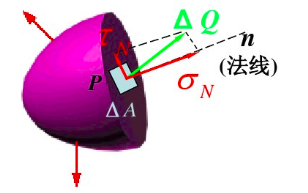
\includegraphics[scale=0.5]{./figures/2.png}
\caption{}
\end{figure}

应力不仅随位置的变化而变化,而且随截面方位的变化而变化。同一点由于截面的法线方向不同,截面上应力也不同。

物体中一点在所有截面上的应力称为该点的应力状态,即通过一点的所有单位面积的内力的集合。
虽然过一点可作无数个平面,但不需要用无数个平面上的应力来描述该点的应力状态,只需用过一点的任意一组相互垂直的三个平面上的应力就可代表该点的应力状态,而其它截面上的应力都可用这组应力与截面的方位关系来表示。

为了表示某一点 $P$ 点的应力状态,引入微分单元体(又称为应力单元,边长分别为 $dx,dy,dz$)

\begin{figure}[H]
\centering
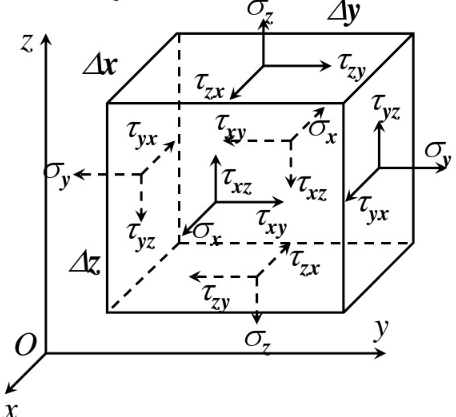
\includegraphics[scale=0.5]{./figures/17.png}
\caption{}
\end{figure}

在坐标系中以 $P$ 点为端点,取与坐标轴平行的平面组成六面体,选取六面体上三个相互垂直的平面,用这三个平面上的应力来描述 $P$ 点的应力状态。

将每一面上的应力分解为一个正应力和两个剪应力,分别与三个坐标轴平行。

正应力用 $\sigma$ 表示,为了表面这个正应力的作用面和作用方向,加上一个下标,例如:正应力 $\sigma_x$ 是作用在垂直于 $x$ 轴的面上,同时也是沿着 $x$ 轴的方向作用的。

剪应力用 $\tau$ 来表示,并加上两个下标,前一个下标表明作用面垂直于哪一个坐标轴,后一个下标表明作用方向沿着哪一个坐标轴。例如:剪应力 $\tau_{xy}$ 是作用在垂直于 $x$ 轴的面上,并且沿着 $y$ 轴的方向作用的。

综上,应力分量的第一个下标表示作用面,第二个下标表示作用方向。正应力的两个下标是一样的,故用一个下标简写。

\begin{figure}[H]
\centering
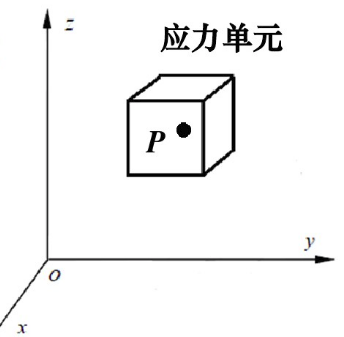
\includegraphics[scale=0.4]{./figures/3.png}
\caption{}
\end{figure}

\begin{figure}[H]
\centering
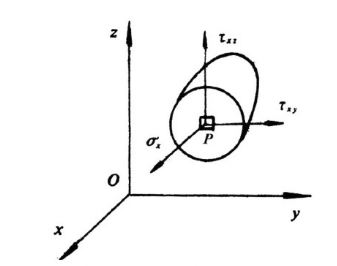
\includegraphics[scale=0.5]{./figures/4.png}
\caption{}
\end{figure}

\begin{figure}[H]
\centering
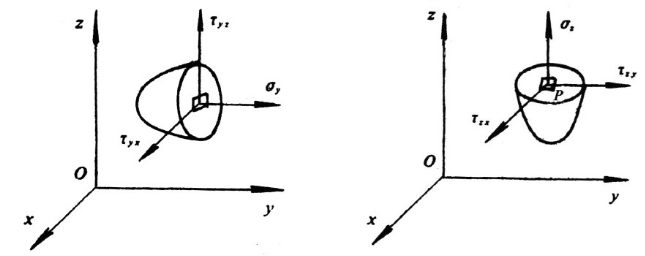
\includegraphics[scale=0.5]{./figures/5.png}
\caption{}
\end{figure}

为判断应力分量的正负号,这里规定:

正面:外法线方向与坐标轴正方向一致;

负面:外法线方向与坐标轴正方向相反;

正面上:应力方向与坐标轴正方向一致时为正;

负面上:应力方向与坐标轴正方向相反时为正;

\begin{figure}[H]
\centering
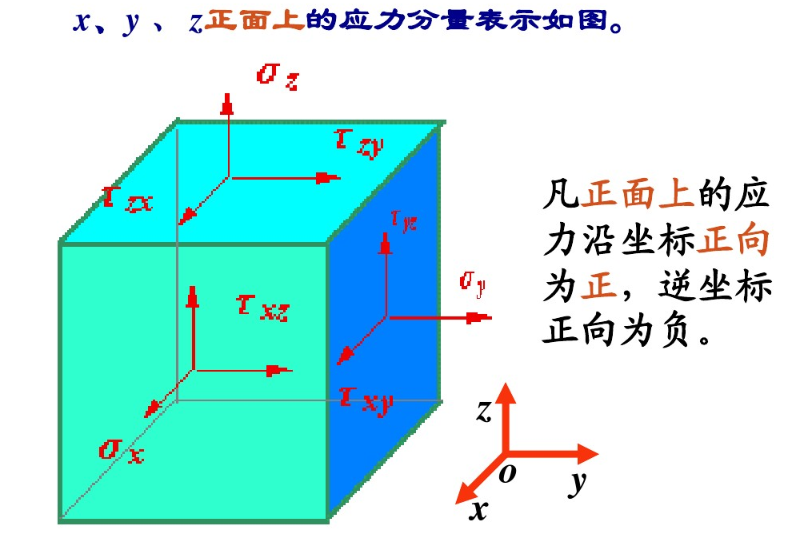
\includegraphics[scale=0.5]{./figures/18.png}
\caption{}
\end{figure}

如果某一个面上的外法线是沿着坐标轴的正方向,这个面上的应力就以沿坐标轴正方向为正,沿坐标轴负方向为负。

相反,如果某一个面上的外法线是沿着坐标轴的负方向,这个面上的应力就以沿坐标轴负方向为正,沿坐标轴正方向为负。

\begin{figure}[H]
\centering
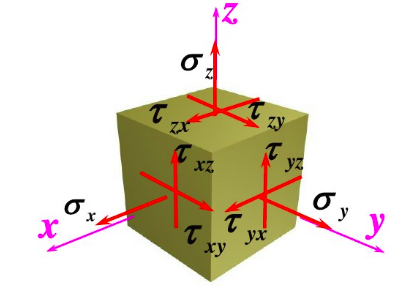
\includegraphics[scale=0.5]{./figures/6.png}
\caption{}
\end{figure}

三个正面上共有九个应力分量(包括三个正应力和六个切应力)。此九个应力分量可写成如下矩阵形式
$$
\begin{bmatrix}
\sigma _x & \tau_{xy} & \tau_{xz} \\
\tau_{yx} & \sigma _y & \tau_{yz} \\
\tau_{zx} & \tau_{zy} & \sigma _z
\end{bmatrix}
$$

张量中,$x \to x_1 , y \to x_2 , z \to x_3$
$$
\sigma _{ij} =
\begin{bmatrix}
\sigma _x & \tau_{xy} & \tau_{xz} \\
\tau_{yx} & \sigma _y & \tau_{yz} \\
\tau_{zx} & \tau_{zy} & \sigma _z
\end{bmatrix}=
\begin{bmatrix}
\sigma _{11} & \sigma_{12} & \sigma_{13} \\
\sigma_{21} & \sigma _{22} & \sigma_{23} \\
\sigma_{31} & \sigma_{32} & \sigma_{33}
\end{bmatrix}
$$

切应力互等定理:作用在相互垂直的两截面上的切应力大小相等。

由于切应力互等定理,上列矩阵中对角的切应力是相等的,即:$\tau_{xy}=\tau_{yx}, \tau_{yz}=\tau_{zy}, \tau_{xz}=\tau_{zx}$,因此,这个矩阵为对称矩阵,并且九个应力分量中只有六个应力分量是独立的。即应力张量是一个对称的二阶张量。

一般来说,弹性体内各点的应力状态都不相同,因此,描述弹性体内应力状态的上述六个应力分量并不是常量,而是 $x,y,z$ 的函数。

已知一点的应力状态,可以求得经过该点的任何截面上的应力。

过 $M$ 点用与坐标平面平行的三个平面截取一微分单元体,在过此单元作一个与 $M$ 点相距为无穷小的任意斜截面。截面 $ABC$ 和过 $M$ 点的单元体平面形成一个微分四面体。知道 $M$ 点的应力状态,以及截面 $ABC$ 与各坐标平面的方向关系,就可求得截面 $ABC$ 上的应力。并且截面 $ABC$ 上的应力可以认为是过 $M$ 点任意截面上的应力。即当截面 $ABC$ 趋近于 $M$ 点时,截面 $ABC$ 上的应力就趋近于经过 $M$ 点的任一斜面上的应力。

\begin{figure}[H]
\centering
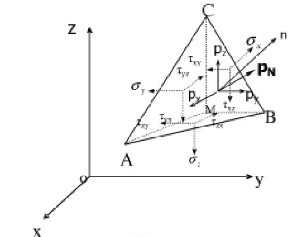
\includegraphics[scale=0.5]{./figures/7.png}
\caption{}
\end{figure}

截面 $ABC$ 外法线向量与各坐标轴正向夹角的方向余弦分别记为 $l,m,n$.

\begin{figure}[H]
\centering
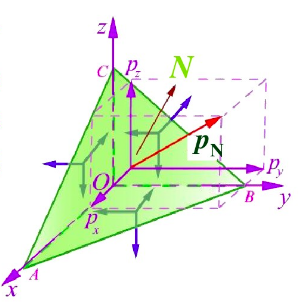
\includegraphics[scale=0.5]{./figures/8.png}
\caption{}
\end{figure}

$\triangle ABC$ 的面积为 $dS$,根据平面图形面积投影定理,$\triangle OAC$ 的面积为 $mdS$,$\triangle OAB$ 的面积为 $ndS$,$\triangle OBC$ 的面积为 $ldS$,
$$
\overrightarrow{p_N}=p_x \overrightarrow{i} +p_y \overrightarrow{j} +p_z \overrightarrow{k}
$$
由$x$轴平衡条件得到
$$
p_x dS-\sigma_x l dS-\tau_{yx}mdS-\tau_{zx}ndS=0
$$
即
$$
p_x -\sigma_x l -\tau_{yx}m-\tau_{zx}n=0
$$
$$
p_x =\sigma_x l +\tau_{yx}m+\tau_{zx}n
$$
同理可得
$$
p_y =\tau_{xy} l +\sigma_x m +\tau_{zy}n
$$
$$
p_z =\tau_{xz} l +\tau_{yz}m + \sigma_z n
$$
写成矩阵形式:
$$
\begin{bmatrix}
p_x \\
p_y \\
p_z
\end{bmatrix}=
\begin{bmatrix}
\sigma _x & \tau_{yx} & \tau_{zx} \\
\tau_{xy} & \sigma _y & \tau_{zy} \\
\tau_{xz} & \tau_{yz} & \sigma _z
\end{bmatrix}
\begin{bmatrix}
l \\
m \\
n
\end{bmatrix}
$$
上式即是平面 $ABC$ 上的应力。

因此,已知应力张量,可以确定任意截面上的应力,当然也就可以确定这个截面上的正应力 $\overrightarrow{\sigma _N}$ 和切应力 $\overrightarrow{\tau_N}$

将 $\overrightarrow{p_N}$ 的各分量向 $\overrightarrow{N}$ 方向投影:
$$
\left|\overrightarrow{\sigma _N}\right|=l\cdot p_x + m\cdot p_y + n\cdot p_z=
\begin{bmatrix}
l & m & n\\
\end{bmatrix}
\begin{bmatrix}
p_x \\
p_y \\
p_z
\end{bmatrix}=
\begin{bmatrix}
l & m & n\\
\end{bmatrix}\sigma _{ij}^T
\begin{bmatrix}
l \\
m \\
n
\end{bmatrix}
$$
切应力:
$$
\left|\overrightarrow{\tau_N}\right|=\sqrt{|\overrightarrow{p_N}|^2-|\overrightarrow{\sigma _N}|^2}
$$

\begin{figure}[H]
\centering
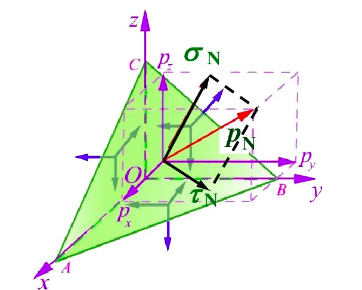
\includegraphics[scale=0.5]{./figures/9.png}
\caption{}
\end{figure}

因此,已知物体内任一点的应力状态,可以求出经过该点的任意斜面上的正应力和切应力。

如果作用在某一截面上的全应力和这一截面垂直,即该截面上只有正应力,切应力为零,则这一截面称为主平面,其法线方向称为应力主方向或应力主轴,其上的应力称为主应力。即 $\overrightarrow{\tau_N}=0$.

\section{应变}
在静力学理论中,通常假定物体是刚性的,即在力的作用下,构成该物体质点之间的距离保持不变。实际上刚体是不存在的,所有物体在某种程度上都是可以变形的,也就是说,在力的作用下,实际物体质点之间的距离总是要发生变化的,一个物体是否可以被假定为刚体,关键在于刚体假定的有效范围。

由于外部因素作用(温度改变等)引起物体内部各质点位置的改变称为位移。物体内任意一点的位移,可以用它 在$x,y,z$三个坐标轴上的投影 $u,v,w$ 来表示,这三个投影称为该点的位移分量。一般来说,位移分量也是 $x,y,z$ 的函数。

位移类别:

刚体位移:位移内部各点位置发生变化,但仍保持初始状态相对位置不变(即物体内任意两点之间距离保持不变)

刚体位移包括平移,转动。

\begin{figure}[H]
\centering
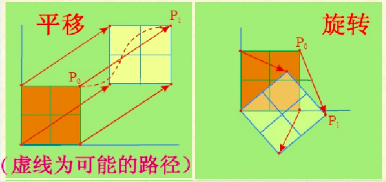
\includegraphics[scale=0.5]{./figures/10.png}
\caption{}
\end{figure}

变形:不仅改变物体的绝对位置,而且改变了物体内部各个点的相对位置,即物体的形状发生改变。

对于弹性力学,主要是研究变形,因为变形的弹性体的应力有着直接的关系。

根据连续性假设,弹性体在变形前和变形后任然保持为连续体。那么弹性体中某点在变形过程中由 $M(x,y,z)$ 移动至 $M'(x',y',z')$,这一过程也将是连续的,$x',y',z'$ 必为 $x,y,z$ 的单值连续函数。设 $MM'=S$ 为位移矢量,其三个分量 $u,v,w$ 为位移分量,则
$$
u=x'(x,y,z)-x=u(x',y',z')
$$
$$
v=y'(x,y,z)-y=v(x',y',z')
$$
$$
w=z'(x,y,z)-z=w(x',y',z')
$$

\begin{figure}[H]
\centering
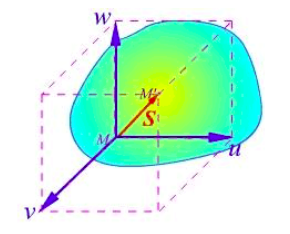
\includegraphics[scale=0.5]{./figures/11.png}
\caption{}
\end{figure}

显然,位移分量 $u,v,w$ 也是 $x,y,z$ 的单值连续函数。

在外力作用下,物体内部任意两点间的相对位置发生改变时,则认为物体发生了变形。物体的变形通常包含:

$1$. ~线段长度的变化

$2$. ~角度的变化

\begin{figure}[H]
\centering
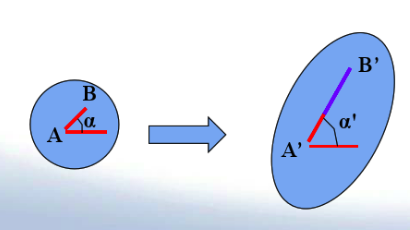
\includegraphics[scale=0.4]{./figures/23.png}
\caption{}
\end{figure}

$$
\varepsilon =\lim\limits_{AB \to 0}\frac{A'B'-AB}{AB}
$$
$$
\gamma = \alpha-\alpha'
$$

\begin{figure}[H]
\centering
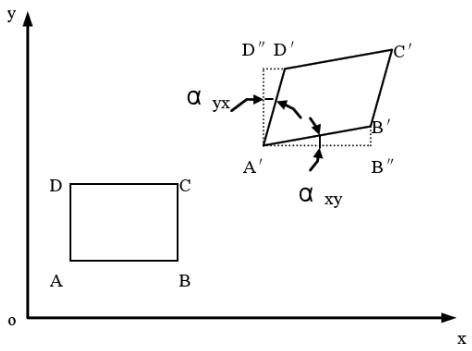
\includegraphics[scale=0.4]{./figures/24.png}
\caption{}
\end{figure}

$$
\varepsilon_x =\lim_{AB \to 0}\frac{A'B''-AB}{AB}
$$
$$
\varepsilon_y =\lim_{AD \to 0}\frac{A'D''-AD}{AD}
$$
$$
\gamma_{xy} =\alpha_{xy}+\alpha_{yx}=\lim\limits_{\substack{AB \to 0 \\ AD \to 0}}(\angle BAD-\angle B'A'D')
$$

物体的变形程度用应变来度量,即应变是表示变形大小的一个物理量。物体变形时,其体内各质点在各方向上都会有应变。应变与位移有密切的联系,位移一旦确定,那么应变也就确定了。

应变与所考虑的点的位置和所选取的方向有关。物体中一点在所有可能方向上的应变的全体称为该点的应变状态。它由通过该点的线段长度的所有变化的总体,以及由该点放射出的任何两条射线之间夹角的所有变化的总体构成。

为了描述弹性体内任一点 $P$ 的应变状态,在这一点沿着坐标轴的正方向取三个微小线段,弹性体变形以后,这三个线段的长度以及它们之间的直角都将改变。表示线段长度的相对伸长或缩短的量称为正应变,线段之间直角的改变称为剪应变。

正应变用 $\varepsilon$ 表示,$\varepsilon_x$ 表示 $x$ 方向的线段的正应变,其余类推。正应变以伸长时为正,缩短时为负。

剪应变用 $\gamma$ 表示,$\gamma_{xy}$ 表示 $x$ 与 $y$ 两方向的线段之间的直角的改变,其余类推。剪应变以直角变小时为正,变大时为负。$\varepsilon_{xy}$ 表示 $x$ 与 $y$ 方向夹角改变量(切应变)的一半,即 $\varepsilon_{xy}=\frac{1}{2}\gamma_{xy}$

虽然棱边 $AB$ 和 $AD$ 偏转的角度不一定相同,但是棱边$AB$ 和 $AD$ 偏转角度之和是 $\gamma_{xy}$,与棱边 $AB$ 和 $AD$ 偏转角度是否相等无关。

\begin{figure}[H]
\centering
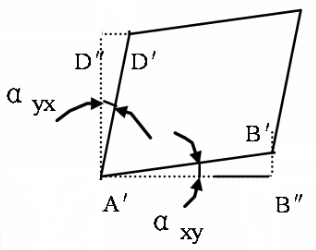
\includegraphics[scale=0.4]{./figures/25.png}
\caption{}
\end{figure}

正应变又叫线应变,它是某一方向上微小线段因变形产生的长度增量(伸长时为正)与原长度的比值。

剪应变又叫角应变或切应变,它是两个相互垂直方向上的微小线段在变形后夹角的改变量(以弧度表示,角度减小时为正)。

~\\

此外,还有一种应变,叫做体应变,定义为单位体积的改变量,一般用 $\theta$ 表示。当体积 $V$ 增大或者缩小时 $\Delta V$ 时,体应变$\theta=\Delta V/V$,无限小应变条件下,
$$
\theta=\varepsilon_x+\varepsilon_y+\varepsilon_z
$$
体应变是由线应变和切应变引起的,并且由上式可知,在无限小应变条件下,体应变只与线应变有关,与切应变无关。

\begin{figure}[H]
\centering
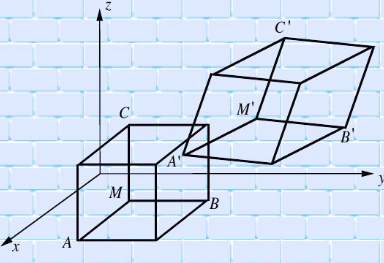
\includegraphics[scale=0.4]{./figures/26.png}
\caption{}
\end{figure}

设单元体的初始边长为 $MA=dx,MB=dy,MC=dz$,变形前的体积为 $V_0=dxdydz$,$x$ 方向上的线应变为 $\varepsilon_x=\frac{r_x-dx}{dx}$,所以 $r_x=dx(1+\varepsilon_x)$.同理,$r_y=dy(1+\varepsilon_y),r_z=dz(1+\varepsilon_z)$.

变形后微小的偏六面体各边边长:

$M'A'=\left(~(1+\varepsilon_x)dx,~ \frac{\partial v}{\partial x}dx,~ \frac{\partial w}{\partial x}dx~\right)$

$M'B'=\left(~\frac{\partial u}{\partial y}dy,~ (1+\varepsilon_y)dy,~ \frac{\partial w}{\partial y}dy~\right)$

$M'C'=\left(~\frac{\partial u}{\partial z}dz,~ \frac{\partial v}{\partial z}dz,~ (1+\varepsilon_z)dz~\right)$

变形后的单元体的体积为

\begin{align*}
V = M'A'\times M'B'\cdot M'C & = \begin{vmatrix}
(1+\varepsilon_x)dx & \frac{\partial v}{\partial x}dx & \frac{\partial w}{\partial x}dx \\
\frac{\partial u}{\partial y}dy & (1+\varepsilon_y)dy & \frac{\partial w}{\partial y}dy \\
\frac{\partial u}{\partial z}dz & \frac{\partial v}{\partial z}dz & (1+\varepsilon_z)dz
\end{vmatrix} \\
& \thickapprox (1+\varepsilon_x)(1+\varepsilon_y)(1+\varepsilon_z)dxdydz \\
& = (1+\varepsilon_x)(1+\varepsilon_y)(1+\varepsilon_z)V_0
\end{align*}

\begin{align*}
\theta=\frac{V-V_0}{V_0} & = \frac{(1+\varepsilon_x)(1+\varepsilon_y)(1+\varepsilon_z)dxdydz-dxdydz}{dxdydz} \\
& = (1+\varepsilon_x)(1+\varepsilon_y)(1+\varepsilon_z)-1 \\
& = \varepsilon_x+\varepsilon_y+\varepsilon_z+\varepsilon_y\varepsilon_z+\varepsilon_z\varepsilon_x+\varepsilon_x\varepsilon_y+\varepsilon_x\varepsilon_y\varepsilon_z \\
& \thickapprox\varepsilon_x+\varepsilon_y+\varepsilon_z=\frac{\partial u}{\partial x}+\frac{\partial v}{\partial y}+\frac{\partial w}{\partial z} 
\end{align*}

略去二阶及以上的高阶微量,得到单元体单位体积的变化(单位体积变化率)

~\\

可以证明一旦已知一点的应变状态,就能计算出通过该点的任一微小线段的正应变,以及经过该点的任意两个微小线段之间的夹角的变化。

与应力分析一样,点的应变状态也是二阶对称张量。它可由一点在三个正交的坐标($x_1,x_2,x_3$)方向的应变分量 $\varepsilon_{ij},(i,j=1,2,3)$ 来确定,其中 $\varepsilon_{11},\varepsilon_{22},\varepsilon_{33}$ 分别为 $x_1,x_2,x_3$ 方向的正应变,而 $\varepsilon_{12}$ 反映 $x_1,x_2$ 两方向上微小线段的夹角改变量(事实上,$\varepsilon_{12}$ 为 $x_1,x_2$ 方向微线段间夹角改变量的一半),其余类推。在九个应变分量 $\varepsilon_{ij}$ 中,$\varepsilon_{ij}=\varepsilon_{ji}$,即只有六个独立分量,它们称为在该点的应变分量。一般来说,应变分量也是 $x,y,z$ 的函数。

把这九个应变分量写成矩阵形式
$$
\varepsilon_{ij}=
\begin{bmatrix}
\varepsilon_{11} & \varepsilon_{12} & \varepsilon_{13} \\
\varepsilon_{21} & \varepsilon_{22} & \varepsilon_{23} \\
\varepsilon_{31} & \varepsilon_{32} & \varepsilon_{33}
\end{bmatrix}=
\begin{bmatrix}
\varepsilon_{x} & \frac{1}{2}\gamma_{xy} & \frac{1}{2}\gamma_{xz} \\
\frac{1}{2}\gamma_{xy} & \varepsilon_{y} & \frac{1}{2}\gamma_{yz} \\
\frac{1}{2}\gamma_{xz} & \frac{1}{2}\gamma_{yz} & \varepsilon_{z}
\end{bmatrix}
$$

在物体内的任一点,如果已知六个应变分量,就可以求出经过该点的任一线段的正应变,也可以求得经过该点的任意两线段之间的夹角的改变。这就是说,六个应变分量完全决定了这一点的应变状态。

应变张量准确描述了物体变形后的局部的几何性质。把应变张量分解为
$$
\begin{bmatrix}
\varepsilon_{11} & \varepsilon_{12} & \varepsilon_{13} \\
\varepsilon_{21} & \varepsilon_{22} & \varepsilon_{23} \\
\varepsilon_{31} & \varepsilon_{32} & \varepsilon_{33}
\end{bmatrix}=\begin{bmatrix}
\varepsilon_{11}-\varepsilon_m & \varepsilon_{12} & \varepsilon_{13} \\
\varepsilon_{21} & \varepsilon_{22}-\varepsilon_m & \varepsilon_{23} \\
\varepsilon_{31} & \varepsilon_{32} & \varepsilon_{33}-\varepsilon_m
\end{bmatrix}+\begin{bmatrix}
\varepsilon_m & 0 & 0 \\
0 & \varepsilon_m & 0 \\
0 & 0 & \varepsilon_m
\end{bmatrix}
$$
其中,$\varepsilon_m=\frac{\varepsilon_{11}+\varepsilon_{22}+\varepsilon_{33}}{3}$ 称为平均正应变,
$\begin{bmatrix}
\varepsilon_{11}-\varepsilon_m & \varepsilon_{12} & \varepsilon_{13} \\
\varepsilon_{21} & \varepsilon_{22}-\varepsilon_m & \varepsilon_{23} \\
\varepsilon_{31} & \varepsilon_{32} & \varepsilon_{33}-\varepsilon_m
\end{bmatrix}$ 反映微元体的形状变化,
$\begin{bmatrix}
\varepsilon_m & 0 & 0 \\
0 & \varepsilon_m & 0 \\
0 & 0 & \varepsilon_m
\end{bmatrix}$ 反映微元体的体积变化。
当应变不一定是无限小时,物体的体积变化不能只是通过$\begin{bmatrix}
\varepsilon_m & 0 & 0 \\
0 & \varepsilon_m & 0 \\
0 & 0 & \varepsilon_m
\end{bmatrix}$ 来反映,因为这个时候的体积变化还与切应变有关。

考虑一个法线为 $\overrightarrow{N}$ 的斜平面,方向余弦 $(l_1=l,l_2=m,l_3=n)$,斜平面上应变 $\overrightarrow{q_N}$:
$$
\begin{bmatrix}
q_{N1} \\
q_{N2} \\
q_{N3}
\end{bmatrix}=
\begin{bmatrix}
\varepsilon_{11} & \varepsilon_{12} & \varepsilon_{13} \\
\varepsilon_{21} & \varepsilon_{22} & \varepsilon_{23} \\
\varepsilon_{31} & \varepsilon_{32} & \varepsilon_{33}
\end{bmatrix}
\begin{bmatrix}
l \\
m \\
n
\end{bmatrix}
$$
如果应变矢量 $\overrightarrow{q_N}$ 在平面法线 $\overrightarrow{N}$ 方向上,即此时剪应变为 $0$,该法线方向即为主方向(或应变主轴),相应的应变称为主应变。

\section{几何方程}
应变分量与位移分量之间有一定的几何关系,这就是所谓的几何方程(用位移导数表示应变)。

对于小变形问题,为了简化分析,将微分单元体分别投影到 $Oxy,Oyz,Ozx$ 平面来讨论。

显然,单元体变形前各棱边是与坐标面平行的,变形后棱边将有相应的转动,但是我们讨论的是小变形问题,这种转动所带来的影响较小。特别是物体位移中不影响变形的计算,假设各点的位移仅为自身的大小和形状的变化所确定,则这种微分线段的转动的误差是十分微小的,不会导致微分单元体的变形有明显的变化。

$oxy$ 平面应变与位移的关系

起于 $P(x,y)$ 点,平行于 $x$ 轴的微元线段 $PQ$(长度$dx$)移动、转动。

\begin{figure}[H]
\centering
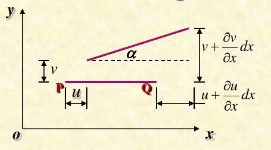
\includegraphics[scale=0.5]{./figures/13.png}
\caption{}
\end{figure}

平行于 $y$ 轴的微元线段 $PT$(长度$dy$)移动、转动。

\begin{figure}[H]
\centering
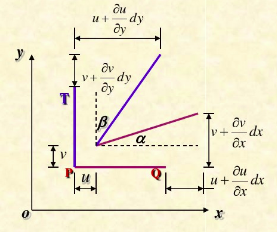
\includegraphics[scale=0.5]{./figures/14.png}
\caption{}
\end{figure}

$P(x,y)$ 点位移是:$(u,v)$,即 $P$ 点 $x$ 方向的位移为 $u(x,y)$,$y$ 方向的位移为$v(x,y)$;
$Q$ 点位移是:$(u',v')$,即 $Q$ 点 $x$ 方向的位移为 $u(x+dx,y)\approx u+\frac{\partial u}{\partial x}dx$,$y$ 方向的位移为$v(x+dx,y)\approx v+\frac{\partial v}{\partial x}dx$;
$T$ 点位移是:$(u'',v'')$,即 $T$ 点 $x$ 方向的位移为 $u(x,y+dy)\approx u+\frac{\partial u}{\partial y}dy$,$y$ 方向的位移为 $v(x,y+dy)\approx v+\frac{\partial v}{\partial y}dy$;
即 $Q$ 点位移为 $(u+\frac{\partial u}{\partial x}dx,v+\frac{\partial v}{\partial x}dx)$,$T$ 点位移为 $(u+\frac{\partial u}{\partial y}dy,v+\frac{\partial v}{\partial y}dy)$

因此,$PQ$ 在 $x$ 方向的正应变:
$$
\varepsilon_x=\frac{(u+\frac{\partial u}{\partial x}dx)-u}{dx}=\frac{\partial u}{\partial x}
$$
转角 $\alpha$:
$$
\alpha=\frac{(v+\frac{\partial v}{\partial x}dx)-v}{dx}=\frac{\partial v}{\partial x}
$$
$tan\alpha\approx\alpha$

$PT$ 在 $y$ 方向的正应变:
$$
\varepsilon_y=\frac{(v+\frac{\partial v}{\partial y}dx)-v}{dy}=\frac{\partial v}{\partial y}
$$
转角 $\beta$:
$$
\beta=\frac{(u+\frac{\partial u}{\partial y}dy)-u}{dy}=\frac{\partial u}{\partial y}
$$
$tan\beta\approx\beta$

因此,正应变为:
$$
\varepsilon_x=\frac{\partial u}{\partial x}, ~ \varepsilon_y=\frac{\partial v}{\partial y}
$$
$P$ 点两直角线段夹角的变化,即剪应变为:
$$
\gamma_{xy}=\alpha +\beta =\frac{\partial v}{\partial x}+\frac{\partial u}{\partial y}
$$
其他平面,结果类似。

$oyz$ 平面:
$$
\varepsilon_z=\frac{\partial w}{\partial z}, ~ \gamma_{yz}=\frac{\partial v}{\partial z}+\frac{\partial w}{\partial y}
$$

$ozx$平面:
$$
\gamma_{zx}=\frac{\partial w}{\partial x}+\frac{\partial u}{\partial z}
$$

最后结果:
$$
\varepsilon_x=\frac{\partial u}{\partial x}, ~ \gamma_{xy}=\frac{\partial u}{\partial y}+\frac{\partial v}{\partial x}
$$
$$
\varepsilon_y=\frac{\partial v}{\partial y}, ~ \gamma_{yz}=\frac{\partial v}{\partial z}+\frac{\partial w}{\partial y}
$$
$$
\varepsilon_z=\frac{\partial w}{\partial z}, ~ \gamma_{zx}=\frac{\partial w}{\partial x}+\frac{\partial u}{\partial z}
$$

上式表明了一点的位移分量和应变分量所应满足的关系,称为几何方程,也称为柯西关系。

矩阵表示:
$$
\varepsilon_{ij}=
\begin{bmatrix}
\varepsilon_{11} & \varepsilon_{12} & \varepsilon_{13} \\
\varepsilon_{21} & \varepsilon_{22} & \varepsilon_{23} \\
\varepsilon_{31} & \varepsilon_{32} & \varepsilon_{33}
\end{bmatrix}=
\begin{bmatrix}
\varepsilon_{x} & \frac{1}{2}\gamma_{xy} & \frac{1}{2}\gamma_{xz} \\
\frac{1}{2}\gamma_{xy} & \varepsilon_{y} & \frac{1}{2}\gamma_{yz} \\
\frac{1}{2}\gamma_{xz} & \frac{1}{2}\gamma_{yz} & \varepsilon_{z}
\end{bmatrix}
$$
$$
\varepsilon_{ij}=
\begin{bmatrix}
\frac{\partial u}{\partial x} & \frac{1}{2}(\frac{\partial v}{\partial x}+\frac{\partial u}{\partial y}) & \frac{1}{2}(\frac{\partial w}{\partial x}+\frac{\partial u}{\partial z}) \\
\frac{1}{2}(\frac{\partial v}{\partial x}+\frac{\partial u}{\partial y}) & \frac{\partial v}{\partial y} & \frac{1}{2}(\frac{\partial w}{\partial y}+\frac{\partial v}{\partial z}) \\
\frac{1}{2}(\frac{\partial w}{\partial x}+\frac{\partial u}{\partial z}) & \frac{1}{2}(\frac{\partial w}{\partial y}+\frac{\partial v}{\partial z}) & \frac{\partial w}{\partial z}
\end{bmatrix}
$$
$\textbf{u}=(u(x,y,z),v(x,y,z),w(x,y,z))$,那么
$$
\nabla\textbf{u}=\begin{bmatrix}
u_x & u_y & u_z \\
v_x & v_y & v_z \\
w_x & w_y & w_z 
\end{bmatrix},~
\nabla\textbf{u}^T=\begin{bmatrix}
u_x & v_x & w_x \\
u_y & v_y & w_y \\
u_z & v_z & w_z 
\end{bmatrix}
$$
因此,
$$
\varepsilon = \frac{1}{2}(\nabla\textbf{u} + \nabla\textbf{u}^T) 
=\begin{bmatrix}
u_x & \frac{v_x + u_y}{2} & \frac{w_x + u_z}{2} \\
\frac{v_x + u_y}{2} & v_y & \frac{w_y + v_z}{2} \\
\frac{w_x + u_z}{2} & \frac{w_y + v_z}{2} & w_z 
\end{bmatrix}
\rightarrow 
\begin{bmatrix}
u_x \\ w_y \\ v_z \\ \frac{w_y + v_z}{2} \\ \frac{w_x + u_z}{2} \\ \frac{v_x + u_y}{2}
\end{bmatrix}
$$

即
$$
\begin{bmatrix}
\varepsilon_{x} & \frac{1}{2}\gamma_{xy} & \frac{1}{2}\gamma_{xz} \\
\frac{1}{2}\gamma_{xy} & \varepsilon_{y} & \frac{1}{2}\gamma_{yz} \\
\frac{1}{2}\gamma_{xz} & \frac{1}{2}\gamma_{yz} & \varepsilon_{z}
\end{bmatrix}=\begin{bmatrix}
u_x & \frac{v_x + u_y}{2} & \frac{w_x + u_z}{2} \\
\frac{v_x + u_y}{2} & v_y & \frac{w_y + v_z}{2} \\
\frac{w_x + u_z}{2} & \frac{w_y + v_z}{2} & w_z 
\end{bmatrix}
$$

上式是在小变形的条件下,由变形的几何关系导出的,称为(小)应变几何方程。由式可知,若已知三个位移分量,则可以确定九个应变分量,其中独立的应变分量只有六个。

使用张量符号,则几何方程可以表示为
$$
\varepsilon_{ij}=\frac{1}{2}(u_{i,j}+u_{j,i})
$$

几何方程表示任一点的微分线段上应变与位移之间的关系。

由几何方程可知,当弹性体的位移分量确定时,应变分量可以通过上式确定;反过来,当应变分量确定时,位移分量却不确定,因为这里涉及到积分,需要确定积分常数,这个可以由边界条件确定。

因此,位移为零或者常数,应变一定为零;应变为零,位移未必为零,物体还可能作刚体位移。也就是说,有应变就有位移,但是有位移不一定就有应变,应变是位置的相对变化决定的。

从物理概念看,各点的位置确定,则微分线段上的应变确定。

从数学推导看,位移函数确定,则其导数(应变)确定。

几何方程的适用条件是: ~ 连续性,小变形;小变形是为了略去高阶小量。

几何方程表示任一点的微分线段应变与位移之间的关系,因此适用于弹性体内的任何点。

\section{静力平衡方程}
沿三坐标轴的正向分别取长度为 $dx$、$dy$ 和 $dz$的三条棱边,由此构成一个微长单元体。同时给这个微六面体施加一个体力 $\textbf{f}=(f_x,f_y,f_z)^T$,微长方体共六个面,有三个正面(“前面”,“上面”,“右面”)和三个负面(“后面”,“下面”,“左面”),每个面上有一个正应力和两个剪应力。并表示出正面上由坐标增量引起的应力增量。

设 $Q(x,y,z)$ 为“后面”上的一点,过 $Q(x,y,z)$ 点的该平面上的应力分量为: $\sigma_x=\sigma_x(x,y,z)$,$\tau_{xy}=\tau_{xy}(x,y,z)$ 和 $\tau_{xz}=\tau_{xz}(x,y,z)$,那么与该平面平行并且相距为 $dx$ 的平面上的应力分量为: $\sigma_x(x+dx,y,z)$,$\tau_{xy}(x+dx,y,z)$ 和 $\tau_{xz}(x+dx,y,z)$,将这三个应力分量作泰勒展式,并略去二次及其以上的小量,得到:
$$
\sigma_x(x+dx,y,z)\approx \sigma_x+\frac{\partial\sigma_x}{\partial x}dx,\tau_{xy}(x+dx,y,z)\approx \tau_{xy}+\frac{\partial\tau_{xy}}{\partial x}dx,\tau_{xz}(x+dx,y,z)\approx \tau_{xz}+\frac{\partial\tau_{xz}}{\partial x}dx
$$
并且这两个平面上的应力方向相反。同理可得其他四个面上的应力分量。

\begin{figure}[H]
\centering
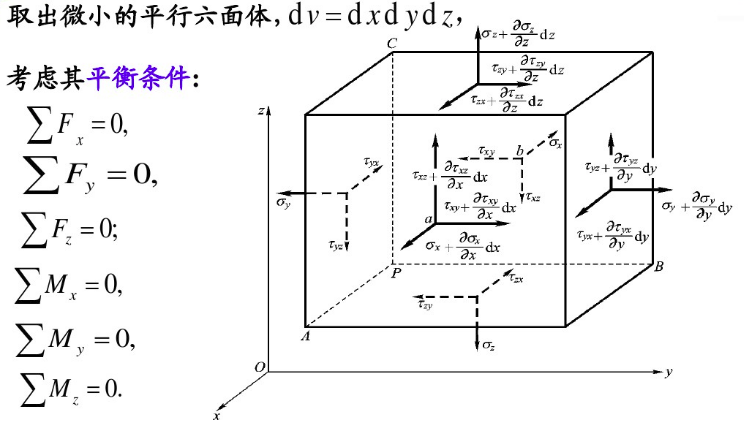
\includegraphics[scale=0.5]{./figures/15.png}
\caption{}
\end{figure}

由 $x$ 方向上力的平衡有
$$
(\sigma_x+\frac{\partial\sigma_x}{\partial x}dx)dydz-\sigma_x dydz+(\tau_{yx}+\frac{\partial\tau_{yx}}{\partial y}dy)dxdz-\tau_{yx}dxdz+(\tau_{zx}+\frac{\partial\tau_{zx}}{\partial z}dz)dxdy-\tau_{zx}dxdy+f_xdxdydz=0
$$
整理得到
$$
\frac{\partial\sigma_x}{\partial x}+\frac{\partial\tau_{yx}}{\partial y}+\frac{\partial\tau_{zx}}{\partial z}+f_x=0
$$
同理可得其他两个方向的平衡方程:
$$
\frac{\partial\tau_{xy}}{\partial x}+\frac{\partial\sigma_{y}}{\partial y}+\frac{\partial\tau_{zy}}{\partial z}+f_y=0
$$
$$
\frac{\partial\tau_{xz}}{\partial x}+\frac{\partial\tau_{yz}}{\partial y}+\frac{\partial\sigma_{x}}{\partial z}+f_z=0
$$
因此,
$$
-\nabla\cdot\begin{bmatrix}
\sigma _x & \tau_{xy} & \tau_{xz} \\
\tau_{yx} & \sigma _y & \tau_{yz} \\
\tau_{zx} & \tau_{zy} & \sigma _z
\end{bmatrix}=\begin{bmatrix}
f_x \\
f_y \\
f_z
\end{bmatrix}
$$

$$
-\nabla\cdot \sigma = \textbf{f}
$$

弹性力学考虑的是微分单元体 $dV$ 的平衡,比理论力学中考虑整体 $V$ 的平衡更加精确;因为当 $dV$ 都平衡时,能够保证 $V$ 平衡,反之不然。

静力平衡方程代表了弹性体内所有点的平衡条件,并且这个平衡条件是精确的。

静力平衡方程表示弹性体内任一点的平衡条件,必然保证了整体的平衡。

静力平衡方程适用条件:~ 连续性,小变形

静力平衡方程中不含 $E,\lambda , \mu , \nu$,方程与材料性质无关。

讨论力矩平衡时,为方便计算,将坐标原点移到微六面体的重心处。由于体力、正应力的合力都通过微六面体的重心,因此它们对三个坐标轴的力矩都为 $0$,力矩平衡方程中仅包含剪应力。

由于剪应力 $\tau_{yx}$ 和 $\tau_{zx}$ 与 $x$ 轴平行,因此对 $x$ 轴的力矩为 $0$,绕 $x$ 轴的力矩平衡方程为:
$$
\tau_{yz}dxdz\cdot\frac{1}{2}dy+(\tau_{yz}+\frac{\partial\tau_{yz}}{\partial y})dxdz\cdot\frac{1}{2}dy-\tau_{zy}dxdy\cdot\frac{1}{2}dz-(\tau_{zy}+\frac{\partial\tau_{zy}}{\partial z})dxdy\cdot\frac{1}{2}dz=0
$$
整理得:
$$
2\tau_{yz}+\frac{\partial\tau_{yz}}{\partial y}dy-2\tau_{zy}-\frac{\partial\tau_{zy}}{\partial z}dz=0
$$
令 $dy\longrightarrow 0,~ dz\longrightarrow 0$,得到 $\tau_{yz}=\tau_{zy}$.

同理可得对于其它两个坐标轴的力矩平衡方程,由此得到:
$$
\tau_{xy}=\tau_{yx}, ~ \tau_{zx}=\tau_{xz}
$$

\section{本构方程}
各向同性材料只有两个独立的材料参数,一般材料的材料参数有六个,统称为拉梅参数,拉梅参数也称为拉梅系数或拉梅常数,用其中任意两个就可以表示其余四个参数。通常,应变-应力关系中的 $\lambda$ 和 $\mu$ 两个材料参数分别称为拉梅的第一个参数和拉梅的第二个参数。

\begin{figure}[H]
\centering
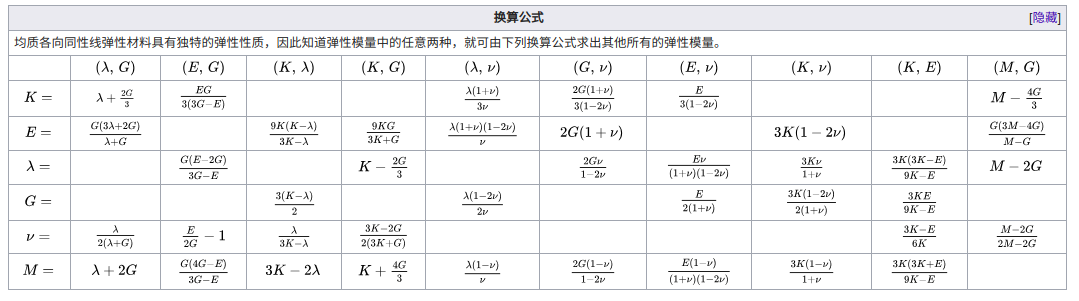
\includegraphics[scale=0.48]{./figures/19.png}
\caption{}
\end{figure}

第一参数 $\lambda$ 没有确切的物理含义,与材料的压缩性有关。在与弹性相关的环境中,$\mu$ 称为剪切模量,有时用 $G$ 表示,而不是$\mu$.通常,符号 $G$ 与使用杨氏模量配对,符号 $\lambda$ 与 $\mu$ 的使用配对。
剪切模量定义为剪应力和剪应变之比:
$$
\mu \text{ or } G = \frac{\tau}{\gamma}
$$ 
它表式材料抵抗切应变的能力。

弹性模量可视为衡量材料产生弹性变形难易程度的指标,其值越大,使材料发生一定弹性变形的应力也越大,即
材料刚度越大,亦即在一定应力作用下,发生弹性变形越小。弹性模量是描述物质弹性的物理量,是一个总称,包括“杨氏模量”、“剪切模量”、“体积模量”等。

杨氏模量是描述固体材料抵抗形变能力的物理量,是弹性模量中最常见的一种。杨氏模量衡量的是一个各向同性弹性体的刚度,它是沿纵向的弹性模量, 定义为正应力和正应变之间的比值。
$$
E = \frac{\sigma}{\epsilon}
$$
杨氏模量是表征材料性质的一
个物理量,仅取决于材料本身的物理性质。杨氏模量的大小标志了材料的刚性,杨氏模量越大,越不容易发生形
变。

体积模量 $K$,用来反映材料的宏观特性,即物体的体应变与平均应力(某一点三个主应力的平均值)之间的关系的一个物理量。

如果材料单向受拉(或受压),那么材料沿载荷方向产生伸长(或缩短)变形的同时,在垂直于载荷的方向会产生缩短(或伸长)变形。垂直载荷方向上的应变 $\varepsilon '$ 与载荷方向上的应变 $\varepsilon$ 之比的负值称为材料的泊松比 $\nu$.

$$
\varepsilon '=-\nu\varepsilon
$$

\begin{figure}[H]
\centering
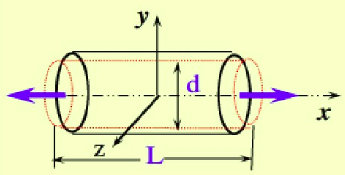
\includegraphics[scale=0.4]{./figures/20.png}
\caption{}
\end{figure}

比如,一杆收拉伸时,其轴向伸长伴随着横向收缩(反之亦然),而横向应变 $\varepsilon '$ 与轴向应变 $\varepsilon$ 之比的负值称为此杆的泊松比 $\nu$.

剪切模量、杨氏模量与泊松比之间的关系:
$$
\lambda = \frac{\nu E}{(1 + \nu)(1 - 2\nu)},\quad \mu \text{ or } G= \frac{E}{2(1 + \nu)}
$$

本构关系: 反映物质宏观性质的数学模型,比如反映力学性质的广义胡克定理。对于不同的物质,在不同的变形条件下有不同的本构关系,也称为不同的本构模型。以下讨论的本构方程都指的是力学中的广义虎克定理(表示应力和应变之间的物理关系)。

\begin{figure}[H]
\centering
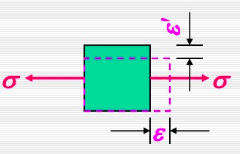
\includegraphics[scale=0.5]{./figures/21.png}
\caption{}
\end{figure}

当弹性体受到一个方向上的简单拉伸(或压缩)时,由杨氏模量的定义有:
$$
\sigma=E\varepsilon
$$
再由泊松比的定义有:
$$
\varepsilon '=-\nu\varepsilon=-\frac{\nu}{E}\sigma
$$

当弹性体受到两个方向上的简单拉伸(或压缩)时

\begin{figure}[H]
\centering
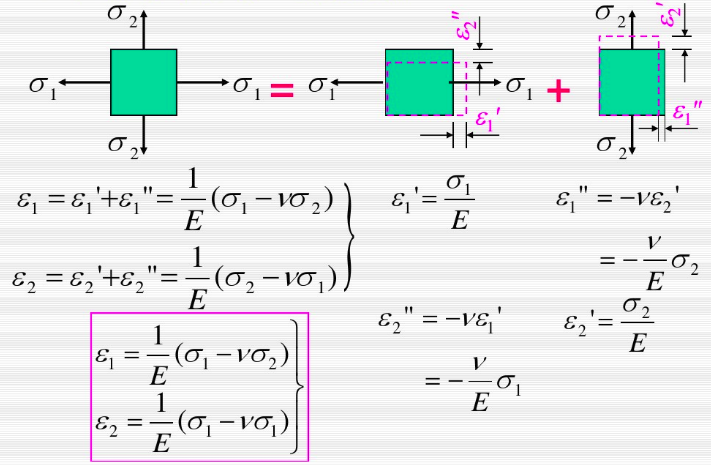
\includegraphics[scale=0.5]{./figures/22.png}
\caption{}
\end{figure}

上式说明正应变 $\varepsilon_1,\varepsilon_2$ 只跟正应力 $\sigma_1,\sigma_2$ 有关,与剪应力无关。

上面就是平面应力状态的广义胡克定律,下面讨论三维的情况。

\begin{figure}[H]
\centering
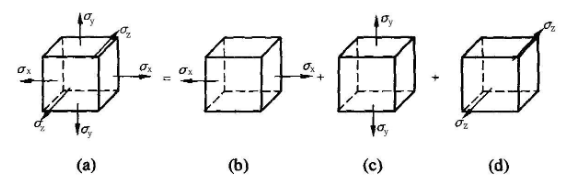
\includegraphics[scale=0.5]{./figures/16.png}
\caption{}
\end{figure}

$x$ 方向受到简单拉伸(没有切应力),由杨氏模量的定义有:
$$
\sigma_x=E\varepsilon'_{x}
$$
因此,当正应力 $\sigma_x$ 单独作用时(图 $(b)$ ),微分单元体在 $x$ 方向上的正应变为
$\varepsilon'_{x}=\frac{\sigma_x}{E}$.

当正应力 $\sigma_y$ 单独作用时(图 $(c)$ ),由泊松比和杨氏模量的定义,微分单元体在 $x$ 方向上的线应变为$\varepsilon''_{x}=-\nu\varepsilon_y=-\nu\frac{\sigma_y}{E}$.

当正应力 $\sigma_z$ 单独作用时(图 $(d)$ ),由泊松比和杨氏模量的定义,微分单元体在 $x$ 方向上的线应变为 $\varepsilon'''_{x}=-\nu\varepsilon_z=-\nu\frac{\sigma_z}{E}$.

在 $\sigma_x,\sigma_y,\sigma_z$ 共同作用下,由叠加原理得到微分单元体在 $x$ 方向上的线应变为
\begin{align*}
\varepsilon_x & =\varepsilon'_{x}+\varepsilon''_{x}+\varepsilon'''_{x} \\
& =\frac{\sigma_x}{E}-\nu\frac{\sigma_y}{E}-\nu\frac{\sigma_z}{E} \\
& =\frac{\sigma_x-\nu(\sigma_y+\sigma_z)}{E}
\end{align*}

同理,可以求得微分单元体在 $y$ 和 $z$ 方向的线应变 $\varepsilon_y$ 和 $\varepsilon_z$
$$
\varepsilon_y=\frac{\sigma_y-\nu(\sigma_x+\sigma_z)}{E}
$$

$$
\varepsilon_z=\frac{\sigma_z-\nu(\sigma_x+\sigma_y)}{E}
$$

当受到纯剪(没有正应力)时,剪应力与剪应变的关系由剪切模量的定义有:
$$
\tau_{xy}=\mu\gamma_{xy}=2\mu\varepsilon_{xy}
$$
如果所有应力都存在,则按叠加原理可得应力-应变关系式(用应力表示应变):
$$
\varepsilon_x=\frac{\sigma_x-\nu(\sigma_y+\sigma_z)}{E}, ~ \varepsilon_y=\frac{\sigma_y-\nu(\sigma_x+\sigma_z)}{E}, ~ \varepsilon_z=\frac{\sigma_z-\nu(\sigma_x+\sigma_y)}{E}
$$

$$
\varepsilon_{xy}=\tau_{xy}/2\mu, ~ \varepsilon_{yz}=\tau_{yz}/2\mu, ~ \varepsilon_{zx}=\tau_{zx}/2\mu
$$
上式就是所谓的本构方程,又称为物理方程。

本构方程:
$$
\varepsilon_x=\frac{\sigma_x-\nu(\sigma_y+\sigma_z)}{E}
$$
$$
\varepsilon_y=\frac{\sigma_y-\nu(\sigma_x+\sigma_z)}{E}
$$
$$
\varepsilon_z=\frac{\sigma_z-\nu(\sigma_x+\sigma_y)}{E}
$$
$$
\varepsilon_{xy}=\tau_{xy}/2\mu ~or~ (~\gamma_{xy}=\tau_{xy}/ \mu~)
$$
$$
\varepsilon_{yz}=\tau_{yz}/2\mu ~or~ (~\gamma_{yz}=\tau_{yz}/ \mu~)
$$
$$
\varepsilon_{zx}=\tau_{zx}/2\mu ~or~ (~\gamma_{zx}=\tau_{zx}/ \mu~)
$$
说明:

$1$. ~ 方程表示了各向同性材料的应力与应变的关系,称为广义 $Hooke$ 定理,也称为本构方程

$2$. ~ 方程组在线弹性条件下成立

或者用应变表示应力,即物理方程的另一种形式是用应变表示的方程
$$
\sigma_x=\frac{E}{(1+\nu)(1-2\nu)}[(1-\nu)\varepsilon_x+\nu(\varepsilon_y+\varepsilon_z)],~ \tau_{xy}=2\mu\varepsilon_{xy}
$$

$$
\sigma_y=\frac{E}{(1+\nu)(1-2\nu)}[(1-\nu)\varepsilon_y+\nu(\varepsilon_x+\varepsilon_z)],~ \tau_{yz}=2\mu\varepsilon_{yz}
$$

$$
\sigma_z=\frac{E}{(1+\nu)(1-2\nu)}[(1-\nu)\varepsilon_z+\nu(\varepsilon_x+\varepsilon_y)],~ \tau_{zx}=2\mu\varepsilon_{zx}
$$

对于线性弹性材料,应力与应变是线性关系
$$
\sigma_x =c_{11}\varepsilon_x+c_{12}\varepsilon_y+c_{13}\varepsilon_z+c_{14}\gamma_{xy}+c_{15}\gamma_{yz}+c_{16}\gamma_{zx}
$$
$$
\sigma_y =c_{21}\varepsilon_x+c_{22}\varepsilon_y+c_{23}\varepsilon_z+c_{24}\gamma_{xy}+c_{25}\gamma_{yz}+c_{26}\gamma_{zx}
$$
$$
\sigma_z =c_{31}\varepsilon_x+c_{32}\varepsilon_y+c_{33}\varepsilon_z+c_{34}\gamma_{xy}+c_{35}\gamma_{yz}+c_{36}\gamma_{zx}
$$
$$
\tau_{xy}=c_{41}\varepsilon_x+c_{42}\varepsilon_y+c_{43}\varepsilon_z+c_{44}\gamma_{xy}+c_{45}\gamma_{yz}+c_{46}\gamma_{zx}
$$
$$
\tau_{yz}=c_{51}\varepsilon_x+c_{52}\varepsilon_y+c_{53}\varepsilon_z+c_{54}\gamma_{xy}+c_{55}\gamma_{yz}+c_{56}\gamma_{zx}
$$
$$
\tau_{zx}=c_{61}\varepsilon_x+c_{62}\varepsilon_y+c_{63}\varepsilon_z+c_{64}\gamma_{xy}+c_{65}\gamma_{yz}+c_{66}\gamma_{zx}
$$

张量形式表示
$$
\begin{bmatrix}
\sigma_{11} \\
\sigma_{22} \\
\sigma_{33} \\
\sigma_{23} \\
\sigma_{31} \\
\sigma_{12} \\
\sigma_{32} \\
\sigma_{13} \\
\sigma_{21}
\end{bmatrix}=
\begin{bmatrix}
C_{1111} & C_{1122} & C_{1133} & C_{1123} & C_{1131} & C_{1112} & C_{1132} & C_{1113} & C_{1121} \\
C_{2211} & C_{2222} & C_{2233} & C_{2223} & C_{2231} & C_{2212} & C_{2232} & C_{2213} & C_{2221} \\
C_{3311} & C_{3322} & C_{3333} & C_{3323} & C_{3331} & C_{3312} & C_{3332} & C_{3313} & C_{3321} \\
C_{2311} & C_{2322} & C_{2333} & C_{2323} & C_{2331} & C_{2312} & C_{2332} & C_{2313} & C_{2321} \\
C_{3111} & C_{3122} & C_{3133} & C_{3123} & C_{3131} & C_{3112} & C_{3132} & C_{3113} & C_{3121} \\
C_{1211} & C_{1222} & C_{1233} & C_{1223} & C_{1231} & C_{1212} & C_{1232} & C_{1213} & C_{1221} \\
C_{3211} & C_{3222} & C_{3233} & C_{3223} & C_{3231} & C_{3212} & C_{3232} & C_{3213} & C_{3221} \\
C_{1311} & C_{1322} & C_{1333} & C_{1323} & C_{1331} & C_{1312} & C_{1332} & C_{1313} & C_{1321} \\
C_{2111} & C_{2122} & C_{2133} & C_{2123} & C_{2131} & C_{2112} & C_{2132} & C_{2113} & C_{2121} 
\end{bmatrix}
\begin{bmatrix}
\varepsilon_{11} \\
\varepsilon_{22} \\
\varepsilon_{33} \\
\varepsilon_{23} \\
\varepsilon_{31} \\
\varepsilon_{12} \\
\varepsilon_{32} \\
\varepsilon_{13} \\
\varepsilon_{21}
\end{bmatrix}
$$

$$
\sigma_{ij}=C_{ijkl}\varepsilon_{kl}
$$
其中 $C_{ijkl}$ 称为四阶弹性张量

根据应力张量和应变张量的对称性,有
$$
C_{ijkl}=C_{jikl}
$$
$$
C_{ijkl}=C_{jilk}
$$

两种表示方式之间的关系

弹性系数 $c$ 的下标 ~~ $1, ~ 2, ~ 3, ~ 4, ~ 5, ~ 6$

对应于张量 $C$ 的指标 ~~ $11, ~ 22, ~ 12, ~ 23, ~ 31$

例如,$c_{11}=C_{1111}, ~ c_{12}=C_{1122}, ~ c_{13}=C_{1133}, ~ c_{14}=C_{1112}$

弹性系数 $c_{mn}$ 也具有对称性
$$
c_{mn}=c_{nm}
$$

其中,

\begin{align*}
\sigma_x & =\frac{E}{(1+\nu)(1-2\nu)}[(1-\nu)\varepsilon_x+\nu(\varepsilon_y+\varepsilon_z)]\\
& =\frac{E}{(1+\nu)(1-2\nu)}[(1-2\nu)\varepsilon_x+\nu(\varepsilon_x+\varepsilon_y+\varepsilon_z)] \\
& =\frac{E}{(1+\nu)}\varepsilon_x+\frac{\nu E}{(1+\nu)(1-2\nu)}(\varepsilon_x+\varepsilon_y+\varepsilon_z) \\
& =2\mu\varepsilon_x+\lambda(\varepsilon_x+\varepsilon_y+\varepsilon_z)
\end{align*}
同理可得,
$$
\sigma_y=2\mu\varepsilon_y+\lambda(\varepsilon_x+\varepsilon_y+\varepsilon_z)
$$

$$
\sigma_z=2\mu\varepsilon_z+\lambda(\varepsilon_x+\varepsilon_y+\varepsilon_z)
$$
因此,
$$
\begin{bmatrix}
\sigma _x & \tau_{yx} & \tau_{zx} \\
\tau_{xy} & \sigma _y & \tau_{zy} \\
\tau_{xz} & \tau_{yz} & \sigma _z
\end{bmatrix}=
\begin{bmatrix}
2\mu\varepsilon_x & 2\mu\varepsilon_{xy} & 2\mu\varepsilon_{xz} \\
2\mu\varepsilon_{yx} & 2\mu\varepsilon_{y} & 2\mu\varepsilon_{yz} \\
2\mu\varepsilon_{zx} & 2\mu\varepsilon_{zy} & 2\mu\varepsilon_{z}
\end{bmatrix}+\begin{bmatrix}
\lambda(\varepsilon_x+\varepsilon_y+\varepsilon_z) &  &  \\
 & \lambda(\varepsilon_x+\varepsilon_y+\varepsilon_z) &  \\
 &  & \lambda(\varepsilon_x+\varepsilon_y+\varepsilon_z)
\end{bmatrix}
$$

$$
\begin{bmatrix}
\sigma _x & \tau_{yx} & \tau_{zx} \\
\tau_{xy} & \sigma _y & \tau_{zy} \\
\tau_{xz} & \tau_{yz} & \sigma _z
\end{bmatrix}=
2\mu\begin{bmatrix}
\varepsilon_x & \varepsilon_{xy} & \varepsilon_{xz} \\
\varepsilon_{yx} & \varepsilon_{y} & \varepsilon_{yz} \\
\varepsilon_{zx} & \varepsilon_{zy} & \varepsilon_{z}
\end{bmatrix}+\begin{bmatrix}
\lambda(\varepsilon_x+\varepsilon_y+\varepsilon_z) &  &  \\
 & \lambda(\varepsilon_x+\varepsilon_y+\varepsilon_z) &  \\
 &  & \lambda(\varepsilon_x+\varepsilon_y+\varepsilon_z)
\end{bmatrix}
$$
简写成
$$
\sigma = 2\mu \varepsilon + \lambda(\t \varepsilon) I
$$

$$
\sigma =
2
\mu
\begin{bmatrix}
u_x & \frac{v_x + u_y}{2} & \frac{w_x + u_z}{2} \\
\frac{v_x + u_y}{2} & v_y & \frac{w_y + v_z}{2} \\
\frac{w_x + u_z}{2} & \frac{w_y + v_z}{2} & w_z 
\end{bmatrix}
+ 
\lambda (u_x + v_y + w_z)
\begin{bmatrix}
1 & 0 & 0 \\
0 & 1 & 0 \\
0 & 0 & 1 
\end{bmatrix}
$$

\begin{align*}
\begin{bmatrix}
\sigma_{11} \\ \sigma_{22} \\ \sigma_{33} \\ \sigma_{23} \\ \sigma_{13} \\ \sigma_{12}
\end{bmatrix} & = \begin{bmatrix}
2\mu u_x + \lambda (u_x + v_y + w_z)\\
2\mu v_y + \lambda (u_x + v_y + w_z)\\
2\mu w_z + \lambda (u_x + v_y + w_z)\\
\mu (w_y + v_z) \\
\mu (w_x + u_z) \\
\mu (v_x + w_y)
\end{bmatrix} \\
& = \begin{bmatrix}
2\mu+\lambda & \lambda & \lambda & 0 & 0 & 0\\
\lambda & 2\mu+\lambda  & \lambda & 0 & 0 & 0\\
\lambda &  \lambda & 2\mu+\lambda & 0 & 0 & 0 \\
0 & 0 & 0 & 2\mu & 0 & 0 \\
0 & 0 & 0 & 0 & 2\mu & 0 \\
0 & 0 & 0 & 0 & 0 & 2\mu
\end{bmatrix}
\begin{bmatrix}
u_x \\ v_y \\ w_z \\ \frac{w_y + v_z}{2} \\ \frac{w_x + u_z}{2} \\ \frac{v_x + u_y}{2}
\end{bmatrix} \\
& = \begin{bmatrix}
2\mu+\lambda & \lambda & \lambda & 0 & 0 & 0\\
\lambda & 2\mu+\lambda  & \lambda & 0 & 0 & 0\\
\lambda &  \lambda & 2\mu+\lambda & 0 & 0 & 0 \\
0 & 0 & 0 & \mu & 0 & 0 \\
0 & 0 & 0 & 0 & \mu & 0 \\
0 & 0 & 0 & 0 & 0 & \mu
\end{bmatrix}
\begin{bmatrix}
\varepsilon_{11} \\ \varepsilon_{22} \\ \varepsilon_{33} \\ 2\varepsilon_{23} \\ 2\varepsilon_{13} \\ 2\varepsilon_{12}
\end{bmatrix} \\
& = \textbf{DB}\begin{bmatrix}
u \\ v \\ w
\end{bmatrix}
\end{align*}

其中,
$$
\textbf{D}=\begin{bmatrix}
2\mu+\lambda & \lambda & \lambda & 0 & 0 & 0 \\
\lambda & 2\mu+\lambda  & \lambda & 0 & 0 & 0 \\
\lambda &  \lambda & 2\mu+\lambda & 0 & 0 & 0 \\
0 & 0 & 0 & \mu & 0 & 0 \\
0 & 0 & 0 & 0 & \mu & 0 \\
0 & 0 & 0 & 0 & 0 & \mu
\end{bmatrix}
$$
$$
\textbf{B}=\begin{bmatrix}
\frac{\partial}{\partial x} & 0 & 0 \\
0 & \frac{\partial}{\partial y}  & 0 \\
0 &  0 &\frac{\partial}{\partial z} \\
0 & \frac{\partial}{\partial z} & \frac{\partial}{\partial y} \\
\frac{\partial}{\partial z} & 0 & \frac{\partial}{\partial x} \\
\frac{\partial}{\partial y} & \frac{\partial}{\partial x} & 0 
\end{bmatrix}
$$

$\textbf{D}$称为弹性矩阵,弹性矩阵是对称矩阵。

本构方程说明,对于各向同性材料,在线弹性、小变形条件下,正应力只引起正应变,切应力只引起切应变。也就说正应变只跟正应力有关,与切应力无关;切应变只跟切应力有关,与正应力无关。

在线弹性力学中,应力与应变的物理关系成线性的广义胡克关系,对于各向同性材料,其中,只有两个弹性常数。

注意这里我们假设材料是线弹性、各向同性的,于是应力与应变的关系是线性的,其中弹性常数只有两个。在各向异性的情况下,上述表达式不再成立,具有更多的弹性常数。

\section{运动平衡方程}
对于处于运动状态的物体,只要加上惯性力,也可以得到平衡方程。惯性力实际上并不存在,因此惯性力又称为假想力。引入了它以后,我们就可以像平衡物体的受力分析那样,对不平衡物体进行“受力分析”。惯性力等于物体的质量乘以加速度并取反方向。

这时,所得方程的形式与前面的静力平衡方程的形式一样,但是应在等式左边加上 $\rho\frac{\partial ^2\textbf{u}}{\partial t^2}$.即
$$
\rho\frac{\partial^2 \textbf{u}}{\partial t^2}-\nabla\cdot \sigma = \textbf{f}
$$
设 $u(x,y,z,t),v(x,y,z,t),w(x,y,z,t)$ 分别表示一点在 $x,y,z$ 方向的位移分量,它们都是点的坐标及时间的函数。再用 $\rho$ 表示弹性体的密度,则对于前面的微分单元体,在三个坐标方向上应分别加上惯性力 
$$-\rho\frac{\partial ^2 u}{\partial t^2}dxdydz,~ -\rho\frac{\partial ^2 v}{\partial t^2}dxdydz,~ -\rho\frac{\partial ^2 w}{\partial t^2}dxdydz
$$
当考虑到这些惯性力时,得到平衡方程
$$
\frac{\partial\sigma_x}{\partial x}+\frac{\partial\tau_{yx}}{\partial y}+\frac{\partial\tau_{zx}}{\partial z}+f_x-\rho\frac{\partial ^2 u}{\partial t^2}=0
$$

$$
\frac{\partial\tau_{xy}}{\partial x}+\frac{\partial\sigma_{y}}{\partial y}+\frac{\partial\tau_{zy}}{\partial z}+f_y-\rho\frac{\partial ^2 v}{\partial t^2}=0
$$

$$
\frac{\partial\tau_{xz}}{\partial x}+\frac{\partial\tau_{yz}}{\partial y}+\frac{\partial\sigma_{x}}{\partial z}+f_z-\rho\frac{\partial ^2 w}{\partial t^2}=0
$$

\section{边界条件}

边界条件:表示边界上的位移约束,或应力与面力之间的关系式,又分为位移边界条件、应力边界条件和混合边界条件。

\begin{figure}[H]
\centering
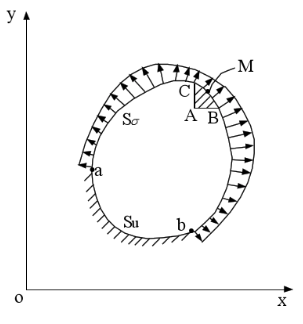
\includegraphics[scale=0.4]{./figures/28.png}
\caption{}
\end{figure}

\subsection{面力边界条件}

若给定了部分边界上的面力分量,则由该部分边界上任意点的静力平衡条件,导出边界上每一点的应力与面力的关系式。可将 $\textbf{应力}$ 中的斜面上的应力分量 $p_x, ~ p_y, ~ p_y$ 分别用面力分量 $F_x, ~ F_y, ~ F_z$ 代替可得。

设 $P$ 为弹性体表面受到面力的区域中的一点,取一包含 $P$ 点的微分四面体,四面体的三个界面平行于坐标平面,斜面为包含 $P$ 点的弹性体表面曲面,也就是说斜面与边界重合。设表面在 $P$ 点的外法线方向 $\textbf{n}_S=(l,m,n)^T$,面力 $\textbf{F}_S=(F_x,F_y,F_z)^T$,斜面面积为 $dS$,那么三个界面的面积分别为 $ldS,mdS,ndS$.如果体力为 $0$,由微分四面体在 $x$ 方向上的力平衡得到
$$
F_xdS-\sigma_xldS-\tau_{yx}mdS-\tau_{zx}ndS=0
$$
即
$$
F_x-\sigma_xl-\tau_{yx}m-\tau_{zx}n=0
$$
同理可得$y,z$ 方向上的力平衡方程为
$$
F_y-\tau_{xy}l-\sigma_{y}m-\tau_{zy}n=0, ~ F_z-\tau_{xz}l-\tau_{yz}m-\sigma_{z}n=0
$$
因此,有
$$
\begin{bmatrix}
F_x \\
F_y \\
F_z
\end{bmatrix}=
\begin{bmatrix}
\sigma _x & \tau_{yx} & \tau_{zx} \\
\tau_{xy} & \sigma _y & \tau_{zy} \\
\tau_{xz} & \tau_{yz} & \sigma _z
\end{bmatrix}
\begin{bmatrix}
l \\
m \\
n
\end{bmatrix}
$$
即
$$
\sigma ^T\textbf{n}_S=\textbf{F}_S=\sigma\textbf{n}_S
$$

\subsection{位移边界条件}
在弹性体的边界上给定位移的约束条件
$$
\textbf{u}=\textbf{u}_S
$$

\section{基本解法}

弹性力学问题共有 $15$ 个方程,即 $3$ 个平衡方程,$6$ 个几何方程,$6$ 个本构方程;求解变量也是 $15$ 个,即 $3$ 个位移分量、$6$ 个应变分量、$6$ 个应力分量。方程的数目恰好等于未知量的数目,因此,在适当的边界条件下,理论上可求解。实际工作中将问题简化,一般以 $3$ 个位移分量或者 $6$ 个应力分量为未知数求解,称为“位移法”或“力法”。

假如已知位移分量,通过几何方程可以得到应变分量,然后通过物理方程可以得到应力分量。反之,如果已知应力分量,也可以通过物理方程得到应变分量,再由几何方程的积分求出位移分量,不过这时的应变分量必须满足一组补充方程,即变形协调方程。

要使几何方程、平衡方程、本构方程有确定的解,还要有对应的面力或位移边界条件。

\subsection{位移法}

以 $3$ 个位移分量为基本未知量,将其它未知量的方程和边界条件用位移来表示。

将几何方程带入本构方程,消去应变分量,得:
$$
\sigma_x = 2\mu\varepsilon_x+\lambda(\varepsilon_x+\varepsilon_y+\varepsilon_z) = 2\mu\frac{\partial u}{\partial x}+\lambda(\frac{\partial u}{\partial x}+\frac{\partial v}{\partial y}+\frac{\partial w}{\partial z})
$$
$$
\sigma_y = 2\mu\varepsilon_y+\lambda(\varepsilon_x+\varepsilon_y+\varepsilon_z) = 2\mu\frac{\partial v}{\partial y}+\lambda(\frac{\partial u}{\partial x}+\frac{\partial v}{\partial y}+\frac{\partial w}{\partial z})
$$
$$
\sigma_z = 2\mu\varepsilon_z+\lambda(\varepsilon_x+\varepsilon_y+\varepsilon_z) = 2\mu\frac{\partial w}{\partial z}+\lambda(\frac{\partial u}{\partial x}+\frac{\partial v}{\partial y}+\frac{\partial w}{\partial z}) 
$$
$$
\tau_{xy} = 2\mu\varepsilon_{xy} = \mu(\frac{\partial u}{\partial y}+\frac{\partial v}{\partial x}) 
$$
$$
\tau_{yz} = 2\mu\varepsilon_{yz} = \mu(\frac{\partial v}{\partial z}+\frac{\partial w}{\partial y}) 
$$
$$
\tau_{zx} = 2\mu\varepsilon_{zx} = \mu(\frac{\partial w}{\partial x}+\frac{\partial u}{\partial z}) 
$$

将各应力带入平衡方程,$x$ 方向的静力平衡方程为:
\begin{align*}
& \frac{\partial\sigma_x}{\partial x}+\frac{\partial\tau_{yx}}{\partial y}+\frac{\partial\tau_{zx}}{\partial z}+f_x \\
& = \lambda\frac{\partial}{\partial x}(\frac{\partial u}{\partial x}+\frac{\partial v}{\partial y}+\frac{\partial w}{\partial z})+2\mu\frac{\partial^2 u}{\partial x^2}+\mu(\frac{\partial^2 u}{\partial y^2}+\frac{\partial^2 v}{\partial x\partial y})+\mu(\frac{\partial ^2 w}{\partial x\partial z}+\frac{\partial ^2 u}{\partial z^2})+f_x \\
& = \lambda\frac{\partial}{\partial x}(\frac{\partial u}{\partial x}+\frac{\partial v}{\partial y}+\frac{\partial w}{\partial z})+\mu(\frac{\partial^2 u}{\partial x^2}+\frac{\partial^2 v}{\partial x\partial y}+\frac{\partial^2 w}{\partial x\partial z})+\mu(\frac{\partial^2 u}{\partial x^2}+\frac{\partial^2 u}{\partial y^2}+\frac{\partial^2 u}{\partial z^2})+f_x \\
& = (\lambda + \mu)\frac{\partial}{\partial x}(\frac{\partial u}{\partial x}+\frac{\partial v}{\partial y}+\frac{\partial w}{\partial z})+\mu\nabla ^2 u+f_x \\
& = 0 \\
\end{align*}
同理:
$$
(\lambda + \mu)\frac{\partial}{\partial y}(\frac{\partial u}{\partial x}+\frac{\partial v}{\partial y}+\frac{\partial w}{\partial z})+\mu\nabla ^2 v+f_y=0
$$
$$
(\lambda + \mu)\frac{\partial}{\partial z}(\frac{\partial u}{\partial x}+\frac{\partial v}{\partial y}+\frac{\partial w}{\partial z})+\mu\nabla ^2 w+f_z=0
$$
上述方程是以位移表示的平衡微分方程,称为拉梅方程。

对于边界条件,如果物体表面的位移已知,则直接由位移形式给定,即使用位移边界条件。

如果给定的边界条件是物体表面的面力,则面力边界条件式需要用位移分量表示,将应力分量带入物理方程,整理可得位移分量表示的面力边界条件:
\begin{align*}
F_x & = \sigma_x l+\tau_{yx}m+\tau_{zx}n \\
& =  \left[2\mu\frac{\partial u}{\partial x}+\lambda(\frac{\partial u}{\partial x}+\frac{\partial v}{\partial x}+\frac{\partial w}{\partial z})\right]l+\mu(\frac{\partial u}{\partial y}+\frac{\partial v}{\partial x})m +\mu(\frac{\partial w}{\partial x}+\frac{\partial u}{\partial z})n \\
& = \lambda(\frac{\partial u}{\partial x}+\frac{\partial v}{\partial y}+\frac{\partial w}{\partial z})l+\mu(\frac{\partial u}{\partial x}l+\frac{\partial u}{\partial y}m+\frac{\partial u}{\partial z}n)+\mu(\frac{\partial u}{\partial x}l+\frac{\partial v}{\partial x}m+\frac{\partial w}{\partial x}n) \\
\end{align*}
同理:
$$
F_y = \lambda(\frac{\partial u}{\partial x}+\frac{\partial v}{\partial y}+\frac{\partial w}{\partial z})l+\mu(\frac{\partial v}{\partial x}l+\frac{\partial v}{\partial y}m+\frac{\partial v}{\partial z}n)+\mu(\frac{\partial u}{\partial y}l+\frac{\partial v}{\partial y}m+\frac{\partial w}{\partial y}n)
$$
$$
F_z = \lambda(\frac{\partial u}{\partial x}+\frac{\partial v}{\partial y}+\frac{\partial w}{\partial z})l+\mu(\frac{\partial w}{\partial x}l+\frac{\partial w}{\partial y}m+\frac{\partial w}{\partial z}n)+\mu(\frac{\partial u}{\partial z}l+\frac{\partial v}{\partial z}m+\frac{\partial w}{\partial z}n)
$$
显然,如果给定的边界条件是面力边界条件,那么位移解法的边界条件表达式十分复杂,因此求解的难度将是比较大的。

总之,如果以位移函数作为基本未知函数求解弹性力学问题,归结为在给定的边界条件下求解位移表示的平衡微分方程,即拉梅方程。

位移分量求解后,则可通过几何方程和物理方程求出相应的应变分量和应力分量。

\subsection{力法}

以应力作为基本未知函数求解弹性力学问题时,应力分量必须满足平衡微分方程和面力边界条件。

但是仅此还不够,仅仅满足上述条件的应力分量并不是真正的应力。因为这组应力分量求出的应变分量代入几何方程,将可能得到一组矛盾方程,不可能求出单值连续的位移分量。要使这组方程不矛盾,则要求应力分量不仅满足平衡微分方程和面力边界条件,而且应力分量对应的应变分量必须满足应变协调方程。

这个问题也可以从物理上解释,应力分量满足平衡微分方程和面力边界条件,只能保证物体的平衡,但是不能保证物体的连续。只有这组应力分量求出的应变分量满足应变协调方程时,才能保证变形后的物体是连续的。

当位移分量作为基本未知函数求解时,应变协调方程是自然满足的。如果位移表示基本未知量,只有应力作为基本未知函数求解时,应变协调方程作为一组补充方程是必须的。

因此,对于应力解法,应力分量必须满足平衡微分方程和应变协调方程。

$\textbf{应变协调方程}$:

平衡方程 — $6$ 个应力分量的 $3$ 个平衡方程

几何方程 — $6$ 个应变分量与 $3$ 个位移分量

由 $6$ 个应变分量求解 $3$ 个位移分量,其方程个数多于未知数个数,方程组要么矛盾,要么相关。由于变形连续,弹性体任意一点的变形必须受到其相邻单元体变形的约束。

应变协调方程 — 反映应变分量之间的关系

$6$ 个应变分量必须满足一定的条件

从几何方程中消去位移分量,第一式和第二式分别对 $y$ 和 $x$ 求二阶偏导数,然后相加,可得:
$$
\frac{\partial^2 \varepsilon_y}{\partial x^2}+\frac{\partial^2 \varepsilon_x}{\partial y^2}=\frac{\partial^2}{\partial x\partial y}(\frac{\partial v}{\partial x}+\frac{\partial u}{\partial y})=\frac{\partial^2 \gamma_{xy}}{\partial x\partial y}
$$

将几何方程的四、五、六式分别对 $z,x,y$,求一阶偏导数,前后两式相加并减去中间一式,则
$$
-\frac{\partial\gamma_{yz}}{\partial x}+\frac{\partial\gamma_{xz}}{\partial y}+\frac{\partial\gamma_{xy}}{\partial z}=2\frac{\partial^2 u}{\partial y\partial z}
$$

对 $x$ 求一阶偏导数,则
$$
\frac{\partial}{\partial x}(--\frac{\partial\gamma_{yz}}{\partial x}+\frac{\partial\gamma_{xz}}{\partial y}+\frac{\partial\gamma_{xy}}{\partial z})=2\frac{\partial^2 \varepsilon_x}{\partial y\partial z}
$$
分别轮换 $x,y,z$,则可得如下 $6$ 个关系式

其中,面内:
$$
\frac{\partial^2 \varepsilon_x}{\partial y^2}+\frac{\partial^2 \varepsilon_y}{\partial x^2}=\frac{\partial^2 \gamma_{xy}}{\partial x\partial y}
$$
$$
\frac{\partial^2 \varepsilon_y}{\partial z^2}+\frac{\partial^2 \varepsilon_z}{\partial y^2}=\frac{\partial^2 \gamma_{yz}}{\partial z\partial y}
$$
$$
\frac{\partial^2 \varepsilon_x}{\partial z^2}+\frac{\partial^2 \varepsilon_z}{\partial x^2}=\frac{\partial^2 \gamma_{zx}}{\partial x\partial z}
$$
面间:

$$
\frac{\partial}{\partial x}(-\frac{\partial\gamma_{yz}}{\partial x}+\frac{\partial\gamma_{zx}}{\partial y}+\frac{\partial\gamma_{xy}}{\partial z})=2\frac{\partial ^2 \varepsilon_x}{\partial y\partial z}
$$
$$
\frac{\partial}{\partial y}(\frac{\partial\gamma_{yz}}{\partial x}-\frac{\partial\gamma_{zx}}{\partial y}+\frac{\partial\gamma_{xy}}{\partial z})=2\frac{\partial ^2 \varepsilon_y}{\partial z\partial x}
$$
$$
\frac{\partial}{\partial z}(\frac{\partial\gamma_{yz}}{\partial x}+\frac{\partial\gamma_{zx}}{\partial y}-\frac{\partial\gamma_{xy}}{\partial z})=2\frac{\partial ^2 \varepsilon_z}{\partial y\partial x}
$$

应变协调方程的数学意义:

使 $3$ 个位移为未知函数的 $6$ 个几何方程不相矛盾

应变协调方程的物理意义:

物体变形后每一单元体都发生形状改变,如果变形不满足一定的关系,变形后的单元体将不能重新合成连续体,其间将产生缝隙或嵌入现象。

为使变形后的物体保持连续体,应变分量必须满足一定的关系

如果不满足应变协调方程,从数学角度看,几何方程矛盾,从物理角度看,弹性体会产生割裂或嵌入现象。

由于变形协调方程是由应变分量表达的,在应力解法中,需要将其转换为由应力分量表达。

将物理方程改写为:
$$
\varepsilon_x=\frac{\sigma_x-\nu(\sigma_y+\sigma_z)}{E}=\frac{1+\nu}{E}\sigma_x-\frac{\nu}{E}(\sigma_x+\sigma_y+\sigma_z),~\gamma_{xy}=\frac{2(1+\nu)}{E}\tau_{xy}
$$
$$
\varepsilon_y=\frac{\sigma_y-\nu(\sigma_x+\sigma_z)}{E}=\frac{1+\nu}{E}\sigma_y-\frac{\nu}{E}(\sigma_x+\sigma_y+\sigma_z),~\gamma_{yz}=\frac{2(1+\nu)}{E}\tau_{yz}
$$
$$
\varepsilon_z=\frac{\sigma_z-\nu(\sigma_x+\sigma_y)}{E}=\frac{1+\nu}{E}\sigma_z-\frac{\nu}{E}(\sigma_x+\sigma_y+\sigma_z),~\gamma_{zx}=\frac{2(1+\nu)}{E}\tau_{zx}
$$
将上式代入变形协调方程的第一、四两式,可得
$$
\frac{\partial^2 \sigma_x}{\partial y^2}+\frac{\partial^2 \sigma_y}{\partial x^2}-\frac{\nu}{1+\nu}\left[\frac{\partial^2 (\sigma_x+\sigma_y+\sigma_z)}{\partial x^2}+\frac{\partial^2 (\sigma_x+\sigma_y+\sigma_z)}{\partial y^2}\right]=2\frac{\partial^2 \tau_{xy}}{\partial x\partial y}
$$
$$
\frac{\partial^2 \sigma_x}{\partial z\partial y}-\frac{\nu}{1+\nu}\frac{\partial^2 (\sigma_x+\sigma_y+\sigma_z)}{\partial y\partial z}=\frac{\partial}{\partial x}(-\frac{\partial\tau_{yz}}{\partial x}+\frac{\partial\tau_{zx}}{\partial y}+\frac{\partial\tau_{xy}}{\partial z})
$$
轮换 $x,y,z$ 可得其余四个方程,由此可得应力表达的变形协调方程。

下面我们对应力分量表示的变形协调方程的两个等式
$$
\frac{\partial^2 \sigma_x}{\partial y^2}+\frac{\partial^2 \sigma_y}{\partial x^2}-\frac{\nu}{1+\nu}\left[\frac{\partial^2 (\sigma_x+\sigma_y+\sigma_z)}{\partial x^2}+\frac{\partial^2 (\sigma_x+\sigma_y+\sigma_z)}{\partial y^2}\right]=2\frac{\partial^2 \tau_{xy}}{\partial x\partial y}
$$
$$
\frac{\partial^2 \sigma_x}{\partial z\partial y}-\frac{\nu}{1+\nu}\frac{\partial^2 (\sigma_x+\sigma_y+\sigma_z)}{\partial y\partial z}=\frac{\partial}{\partial x}(-\frac{\partial\tau_{yz}}{\partial x}+\frac{\partial\tau_{zx}}{\partial y}+\frac{\partial\tau_{xy}}{\partial z})
$$
作简化。

首先对平衡微分方程的第二和第三两式分别对 $z,y$ 求偏导数,然后相加可以得到
$$
\frac{\partial^2 \tau_{xy}}{\partial x\partial z}+\frac{\partial^2 \sigma_y}{\partial y\partial z}+\frac{\partial^2 \tau_{yz}}{\partial z^2}+\frac{\partial^2 \tau_{xz}}{\partial x\partial y}+\frac{\partial^2 \tau_{yz}}{\partial y^2}+\frac{\partial^2 \varepsilon_z}{\partial y\partial z}=-(\frac{\partial f_x}{\partial y}+\frac{\partial f_y}{\partial z})
$$
将上式与上面的变形协调方程两个等式中的第二个式子相加后并整理,可得
$$
\nabla^2\tau_{yz}+\frac{1}{1+\nu}\frac{\partial^2 (\sigma_x+\sigma_y+\sigma_z)}{\partial y\partial z}=-(\frac{\partial f_y}{\partial z}+\frac{\partial f_z}{\partial y})
$$
上式为简化后的方程,轮换 $x,y,z$ 以后,可得另外两个类似的公式

综上所述,我们一共得到以下六个关系式:
$$
\nabla^2\sigma_x-\frac{1}{1+\nu}\frac{\partial^2 (\sigma_x+\sigma_y+\sigma_z)}{\partial x^2}=-\frac{\nu}{1-\nu}(\frac{\partial f_x}{\partial x}+\frac{\partial f_y}{\partial y}+\frac{\partial f_z}{\partial z})-2\frac{\partial f_x}{\partial x}
$$
$$
\nabla^2\sigma_y-\frac{1}{1+\nu}\frac{\partial^2 (\sigma_x+\sigma_y+\sigma_z)}{\partial y^2}=-\frac{\nu}{1-\nu}(\frac{\partial f_x}{\partial x}+\frac{\partial f_y}{\partial y}+\frac{\partial f_z}{\partial z})-2\frac{\partial f_y}{\partial y}
$$
$$
\nabla^2\sigma_x-\frac{1}{1+\nu}\frac{\partial^2 (\sigma_x+\sigma_y+\sigma_z)}{\partial z^2}=-\frac{\nu}{1-\nu}(\frac{\partial f_x}{\partial x}+\frac{\partial f_y}{\partial y}+\frac{\partial f_z}{\partial z})-2\frac{\partial f_z}{\partial z}
$$
$$
\nabla^2\tau_{xy}+\frac{1}{1+\nu}\frac{\partial^2 (\sigma_x+\sigma_y+\sigma_z)}{\partial x\partial y}=-(\frac{\partial f_y}{\partial x}+\frac{\partial f_x}{\partial y})
$$
$$
\nabla^2\tau_{yz}+\frac{1}{1+\nu}\frac{\partial^2 (\sigma_x+\sigma_y+\sigma_z)}{\partial y\partial z}=-(\frac{\partial f_y}{\partial z}+\frac{\partial f_z}{\partial y})
$$
$$
\nabla^2\tau_{zx}+\frac{1}{1+\nu}\frac{\partial^2 (\sigma_x+\sigma_y+\sigma_z)}{\partial z\partial x}=-(\frac{\partial f_x}{\partial z}+\frac{\partial f_z}{\partial x})
$$

上述方程即为应力分量表达的应变协调方程,但是应该注意:应力是不需要协调的,其实质仍为应变分量所满足的变形协调关系。

总而言之,在以应力函数作为基本未知量求解时,归结为在给定的边界条件下,求解平衡微分方程和应力表达的变形协调方程所组成的偏微分方程组。

\subsection{混合解法}

混合解法以 $6$ 个应力分量和 $3$ 个位移分量作为基本未知量求解弹性力学问题。通过物理方程中消去应变分量,其基本方程为平衡微分方程和由应力分量表达的几何方程,即
$$
\frac{\partial u}{\partial x}=\frac{1}{E}\left[(1+\nu)\sigma_x-\nu(\sigma_x+\sigma_y+\sigma_z)\right], ~~ \frac{\partial v}{\partial x}+\frac{\partial u}{\partial y}=\frac{2(1+\nu)}{E}\tau_{xy}
$$
$$
\frac{\partial v}{\partial y}=\frac{1}{E}\left[(1+\nu)\sigma_y-\nu(\sigma_x+\sigma_y+\sigma_z)\right], ~~ \frac{\partial w}{\partial y}+\frac{\partial v}{\partial z}=\frac{2(1+\nu)}{E}\tau_{yz}
$$
$$
\frac{\partial w}{\partial z}=\frac{1}{E}\left[(1+\nu)\sigma_z-\nu(\sigma_x+\sigma_y+\sigma_z)\right], ~~ \frac{\partial u}{\partial z}+\frac{\partial w}{\partial x}=\frac{2(1+\nu)}{E}\tau_{zx}
$$

这里有 $3$个平衡微分方程和 $6$个几何方程,共计 $9$ 个方程对应 $9$个未知函数,加上给定的边界条件,则可得到唯一的解。

弹性力学的基本求解方法的应用要根据问题性质,主要是根据边界条件选择使用。

对于面力边界条件问题,使用应力解法;位移边界条件应用位移解法;混合解法主要应用于混合边界条件,即弹性体的部分边界位移已知,部分边界面力已知的问题。


为了证明弹性力学解的唯一性定理,首先证明一个重要的定理,即应变能定理。

应变能定理是指:弹性体在外力作用下处于平衡状态时,物体内存储的弹性势能,即应变能,等于外力由原始位置到平衡位置所做的功。假如外力是由 $0$ 连续变化到其最终数值的,则在加载的过程中,物体始终是处于平衡状态的。

以下证明弹性体的应变能定理。设弹性体处于体力 $f_x, f_y, f_z$ 和面力 $F_x, F_y, F_z$ 的作用下,弹性体内产生位移 $u,v,w$.则外力在位移过程中作功为
$$
W=\frac{1}{2}\iiint\limits_V (f_x u+f_y v+f_z w)dV+\frac{1}{2}\iint\limits_S (F_x u+F_y v+F_z w)dS
$$

将面力边界条件代入上式的第二个积分,并利用高斯积分公式,可得

$W=$
$$
\frac{1}{2}\iiint\limits_V \left[(\frac{\partial \sigma_x}{\partial x}+\frac{\partial \tau_{xy}}{\partial y}+\frac{\partial \tau_{zx}}{\partial z}+f_x)u+(\frac{\partial \tau_{xy}}{\partial x}+\frac{\partial \sigma_y}{\partial y}+\frac{\partial \tau_{yz}}{\partial z}+f_y)v+(\frac{\partial \tau_{zx}}{\partial x}+\frac{\partial \tau_{yz}}{\partial y}+\frac{\partial \sigma_z}{\partial z}+f_z)w\right]dV
$$
$$
+ \frac{1}{2}\iiint\limits_V \left[\sigma_x\frac{\partial u}{\partial x}+\sigma_y\frac{\partial v}{\partial y}+\sigma_z\frac{\partial w}{\partial z}+\tau_{xy}(\frac{\partial v}{\partial x}+\frac{\partial u}{\partial y})+\tau_{yz}(\frac{\partial w}{\partial y}+\frac{\partial v}{\partial z}+\tau_{zx}(\frac{\partial u}{\partial z})+\frac{\partial w}{\partial x})\right]dV
$$
$
= \frac{1}{2}\iiint\limits_V (\sigma_x\varepsilon_x+\sigma_y\varepsilon_y+\sigma_z\varepsilon_z+\tau_{xy}\gamma_{xy}+\tau_{yz}\gamma_{yz}+\tau_{zx}\gamma_{zx})dV
$

由此可以证明,外力所做的功等于弹性体存储的弹性势能。

对于一般的工程构件,即弹性体,由于偏微分方程边值问题在数学上求解的困难,因此直接根据给定的边界条件求解弹性力学的基本方程是十分困难的。

为了避开偏微分方程边值问题直接求解的困难,在弹性力学问题的求解中,经常采用的方法是逆解法和半逆解法。

解的唯一性定理: ~ 弹性力学基本方程(几何方程、平衡方程、本构方程)在给定边界条件的情况下,其解是唯一的。

解的唯一性定理可以简化弹性力学问题的求解,它是逆解法、半逆解法的理论依据。

逆解法: ~ 预先选取一组位移或应力函数,然后验证其满足弹性基本方程和边界条件,该组函数即为问题的解。

半逆解法: ~ 在所有的未知量中,预先假设一部分已知,另一部分则根据基本方程和边界条件求出,从而得到全部的未知量。

逆解法和半逆解法的求解过程带有“试算”的性质。

解的迭加原理: ~ 弹性力学解的迭加原理是指在线弹性条件下,对于满足小变形条件的弹性体,在两组不同的外力作用下所得到的弹性力学解相加等于这两组外力共同作用于弹性体的解答。

小变形、线弹性变形是叠加原理成立的条件。大变形时位移和应变之间是非线性关系,塑性情况下应力和应变之间是非线性关系,因此都不适用叠加原理。

~ \\

弹性力学问题的求解是在给定的边界条件下求解基本方程。由于偏微分方程边值问题的性质,弹性力学的解必然要求物体表面的外力或者位移是按一定的规律分布的。对于工程实际问题,构件表面面力或者位移是很难满足这个要求的。这使得弹性力学解的应用将受到极大的限制。

为了扩大弹性力学解的适用范围,放宽这种限制,圣维南提出了局部影响原理。

圣维南局部影响原理其主要内容为:

 作用在弹性体表面局部面积上的力系,如果被同一作用面上的等效力系所代替,只会影响与载荷作用处很近处的应力,对载荷较远处只有极小的影响。

根据圣维南局部影响原理,假如我们用一等效力系取代弹性体上作用的原外力,则其影响仅在力的作用区域附近。离此区域较远处,几乎不受影响。

\begin{figure}[H]
\centering
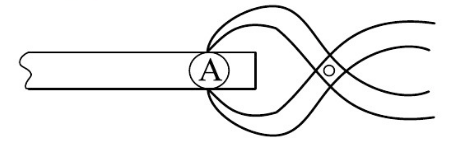
\includegraphics[scale=0.4]{./figures/27.png}
\caption{}
\end{figure}

上图钳子夹住一根直杆,那么直杆上加上了一组平衡力系,实验证明,无论作用的力有多大,在 $A$ 区域以外的应力很小,这一现象可以用圣维南原理来解释。







%坎坎坷坷扩


%\cite{tam19912d}
%\bibliography{../ref}
\end{document}
